
\chapter{Mixed Finite Element Methods}\label{chap7}

\section{The Abstract Continuous Problem}\label{chap7:ssec7.1}
Let\pageoriginale $V,M,H$ be Hilbert spaces with $V\hookrightarrow
H$. The continuous problem is:   

Find $\{u,\lambda\}\;\varepsilon V\times M$ such that 
\begin{align*}
&a(u,v)+b(v,\lambda) = (f,v)\; \; \forall \; v\; \varepsilon
V,\tag{7.1}\label{chap7:eq7.1} \\
&b(u,\mu) = (\phi,\mu)\; \; \forall \;\mu \; \varepsilon
M,\tag{7.1b}\label{chap7:eq7.1b} 
\end{align*} 
where $a(\cdotp,\cdotp):H\times H\to\mathbb{R}$ and
$b(\cdotp,\cdotp):V\times M\to\mathbb{R}$ are continuous bilinear
forms and $f\varepsilon V', \phi\varepsilon M'$. 

Let $a(\cdotp,\cdotp)$ and $b(\cdotp,\cdotp)$ satisfy
\begin{align*}
&a(v,v)\geq\alpha\parallel v\parallel_H^2\forall \; v \;\varepsilon H
\quad\text{ellipticity},\tag{7.2}\label{chap7:eq7.2}\\
&\underset{v\varepsilon V}{\Sup}\frac{b(v,\mu)} {\parallel v\parallel_V}
\geq \beta\parallel\mu\parallel_M\quad \text{Brezzi's
condition}\tag{7.3} \label{chap7:eq7.3} 
\end{align*}
$|a(u,v)|\leq |a|\parallel u\parallel \parallel v\parallel$,
$|b(v,\mu)|\leq |b|\parallel v\parallel \parallel \mu\parallel$. We
have 

\setcounter{THM}{0}
\begin{THM}\label{chap7:THM1}
If $H=V$ then, under the above assumptions problem
\eqref{chap7:ssec7.1} has a unique solution.
\end{THM}

\begin{proof}
Let us consider the regularised problem:
\begin{align*}
& a(u_\varepsilon,v)+b(v,\lambda_\varepsilon)=(f,v)\;\; \forall\;v\;\varepsilon
\;V,\tag{7.4}\label{chap7:eq7.4} \\
& -b(u_\varepsilon,\mu)+\varepsilon(\lambda_\varepsilon,\mu)=-(\phi,\mu)\; \; \forall
\;\mu\;\varepsilon M,\tag{7.4b}\label{chap7:eq7.4b}
\end{align*}
Let $\Phi =\{u,\lambda\}, \Psi =\{v,\mu\}\varepsilon V\times M$. We
define 
$$
A_\varepsilon(\Phi,\Psi)=a(u,v)+b(v,\lambda)-b(u,\mu)+\varepsilon(\lambda,
\mu), L(\Psi)=(f,v)-(\phi,\mu)
$$
Then\pageoriginale $A_\varepsilon(\Phi,\Psi)$ is $V\times M$ coercive
and $L(\Psi)$ is a continuous, linear form on $V\times M$.

It is easy to see that problem \eqref{chap7:eq7.4} is equivalent to:
\setcounter{equation}{4}
\begin{equation}\label{chap7:eq7.5}
\left.
\begin{aligned}
\text{Find}\quad\Phi\varepsilon V\times M\quad\text{such that}\\
A_\varepsilon(\Phi,\Psi)=L(\Psi) \; \forall \; \Psi\varepsilon V\times M
\end{aligned} 
\right\}
\end{equation}
By Lax-Milgram Lemma, problem \eqref{chap7:eq7.5} has a unique
solution which implies that the regularized problem
\eqref{chap7:eq7.4} has a unique solution. 

Taking $v=u_\varepsilon$ in \eqref{chap7:eq7.4}, $\mu=\lambda_\varepsilon$ in
\eqref{chap7:eq7.4b} and adding and using the continuity of bilinear forms and
$H$-ellipticity of $a(\cdotp,\cdotp)$, we get 
\begin{equation}\label{chap7:eq7.6}
\alpha\parallel u_\varepsilon\parallel^2+\varepsilon\parallel
\lambda_\varepsilon\parallel^2\leq C\left(\parallel u_\varepsilon
\parallel +\parallel\lambda_\varepsilon\parallel\right),
\end{equation}
where $C$ is a constant.

Since
$$
b(v,\lambda_\varepsilon)=(f,v)-a(u_\varepsilon,v)\leq\left(\parallel
f\parallel_* +|a|\parallel u_\varepsilon\parallel\right)\parallel
v\parallel 
$$
we obtain, using Brezzi's condition, 
$$
\beta\parallel\lambda_\varepsilon\parallel\leq\underset{v\varepsilon V}
{\Sup}\; \frac{b(v,\lambda_\varepsilon)}{\parallel v\parallel}\leq
\parallel f\parallel_*+|a|\parallel u_\varepsilon\parallel.
$$
This implies 
\begin{equation}\label{chap7:eq7.7}
\parallel\lambda_\varepsilon\parallel\leq C\left(1+\parallel
u_\varepsilon \parallel\right).
\end{equation}
From \eqref{chap7:eq7.6} and \eqref{chap7:eq7.7} we obtain 
$$
\parallel u_\varepsilon \parallel \leq C\quad\text{and}\quad \parallel
\lambda_\varepsilon\parallel\leq C,
$$
where\pageoriginale $C$ is a constant. Hence there exists a
subsequence $\{\in'\}$, $u\in V$, $\lambda\in M$,
such that 
$$
u_{\in'}\rightharpoonup u\quad\text{and}\quad
\lambda_{\in'}\rightharpoonup\lambda.
$$
Obviously $\{u,\lambda\}$ is a solution of \eqref{chap7:eq7.1}.

If $\{u_1,\lambda_1\}$ and $\{u_2,\lambda_2\}$ are solutions of
\eqref{chap7:eq7.1}, then 
\begin{equation}\label{chap7:eq7.8}
\begin{split}
a(u_1-u_2,v)+b(v,\lambda_1-\lambda_2)=0 \; \forall v\in V,\\
b(u_1-u_2,\mu)=0 \; \forall\mu\in M.
\end{split}
\end{equation}
Taking $v=u_1-u_2$ and $\mu=\lambda_1-\lambda_2$, we obtain 
$$
\alpha\parallel u_1-u_2\parallel^2\leq a(u_1-u_2,u_1-u_2)=0.
$$
Therefore
$$
u_1=u_2.
$$

Since $u_1=u_2$, using Brezzi's condition, we obtain from
\eqref{chap7:eq7.8} that 
$$
\lambda_1=\lambda_2.
$$

Hence the solution of \eqref{chap7:eq7.1} is unique.
\end{proof}

\setcounter{REM}{0}
\begin{REM}\label{chap7:rem1}
We now give an error estimate for the solution of \eqref{chap7:eq7.1}
and the regularized problem \eqref{chap7:eq7.4}. We have 
$$
a(u-u_\varepsilon,v)+b(v,\lambda -\lambda_\varepsilon)=0 \; \forall
v\in V.
$$
Hence 
\begin{equation}\label{chap7:eq7.9}
\beta\parallel\lambda -\lambda_\in\parallel\leq |a|. \parallel
u-u_\in \parallel.
\end{equation}

From \eqref{chap7:eq7.1b} and \eqref{chap7:eq7.4b} we obtain
$$
b(u-u_\in,\mu)+\in(\lambda_\in,\mu)=0\forall
\mu\in M.
$$\pageoriginale
Choosing $v=u-u_\in,\mu=\lambda-\lambda_\in$, we get 
$$
\alpha\parallel u-u_\in\parallel^2\leq a(u-u_\in,
u-u_\in)=\in(\lambda_\in,\lambda-\lambda_\in)
\leq\in\parallel\lambda_\in\parallel \parallel\lambda
-\lambda_\in\parallel
$$
Thus, using \eqref{chap7:eq7.7}
$$
\parallel u-u_\in\parallel \leq C\in.
$$
Thus from \eqref{chap7:eq7.9} we get 
$$
\parallel\lambda-\lambda_\in\parallel\leq C\in.
$$
So we obtain
$$
\parallel u-u_\in\parallel=0(\in)\quad\text{and}\quad
\parallel\lambda-\lambda_\in\parallel=0(\in).
$$
\end{REM}

\begin{REM}\label{chap7:rem2}
Let $B:V\to M$ be such that 
$$
(Bv,\mu)_M=b(v,\mu)\;\forall\;\mu\;\in\; M.
$$
One has, from \eqref{chap7:eq7.4b} and \eqref{chap7:eq7.4},
\begin{gather*}
\lambda_\in= 1/\in\;(Bu_\in-\phi),\\
a(u_\in,v)+1/\in\;(Bv, Bu_\in-\phi)=
(f,v)\;\forall\;v\;\in \;V,
\end{gather*}
which correspond to penalization of \eqref{chap7:eq7.1b}.
\end{REM}

\begin{REM}\label{chap7:rem3}
We proved the existence and uniqueness of \eqref{chap7:eq7.1} only
under the assumption $V=H$. If $V\neq H$ then we do not have a
general existence theorem. But existence theorems for particular
examples when $V\neq H$ are proved.

We now give examples of \eqref{chap7:eq7.1}. 
\end{REM}

\setcounter{exam}{0}
\begin{exam}\label{chap7:exm1}
{\bf The\pageoriginale Stokes Problem.} We recall that the Stokes
problem is: 

Find $\{u,p\}$ such that 
\begin{align*}
-\gamma\Delta u+\nabla p &= f\quad\text{in}\quad\Omega,\\
\Div u &= 0\quad\text{in}\quad\Omega,\\
u &= 0\quad\text{on}\quad\Gamma.
\end{align*}

Without loss of generality we can take $\gamma =1$. Using the standard
technique of integration by parts we find that this corresponds to the
problem:

Find
$$
\{u,p\}\;\varepsilon\;(H_\circ^1(\Omega))^n\;\times\;(L^2(\Omega)/
\mathbb{R})
$$
such that 
\begin{align*}
a(u,v)+b(v,p) &= (f,v)\;\forall\;v\;\varepsilon\;(H_\circ^1
(\Omega))^n,\\ 
b(u,\mu) &= 0\;\forall\;\mu\;\varepsilon\;L^2(\Omega)/\mathbb{R};
\end{align*}
where
\begin{align*}
a(u,v) &= \int\limits_\Omega\nabla u.\nabla v\,dx,\\
b(v,\mu) &= -\int\limits_\Omega\mu\;\Div\;v\,dx.
\end{align*}
We take
\begin{align*}
V &= H=(H_\circ^1(\Omega))^n,\\
M &= (L^2(\Omega)/\mathbb{R}).
\end{align*}
Clearly $a(\cdotp,\cdotp)$ is $H$-elliptic, continuous and
bilinear. Let us prove\break Brezzi's condition, 
\begin{gather*}
\underset{v\varepsilon V}{\Sup}\frac{b(v,\lambda)}{\parallel
v\parallel_V}=\underset{v\varepsilon(H_\circ^1(\Omega))^n}{\Sup}
\frac{-\int\limits_\Omega\lambda\Div\;v}{\parallel v\parallel_V}=
\underset{v\varepsilon(H_\circ^1(\Omega))^n}{\Sup}
\frac{<\nabla\lambda,v>}{\parallel v\parallel_V}\\
=\parallel\nabla\lambda\parallel_{(H^{-1}(\Omega))^n}\geq\frac{1}{C}
\parallel\lambda\parallel_{L^2(\Omega)/\mathbb{R}}
\end{gather*}\pageoriginale
where $\langle , \rangle$ denotes the duality between $(H_\circ^1(\Omega))^n$ and
$(H^{-1}(\Omega))^n$. 

Thus Stokes problem has a unique solution. 
\end{exam}

\begin{exam}\label{chap7:exm2}
{\bf The Biharmonic Problem.} Let 
$$
V=H^1(\Omega),\;M=H_\circ^1(\Omega),\;H=L^2(\Omega).
$$
Consider the problem:

Find
$$
\{u,\lambda\}\;\varepsilon\;H^1(\Omega)\;\times\;H_\circ^1(\Omega)
$$
such that 
\begin{align}
& a(u,v)+b(v,\lambda)=0\; \; \forall\;v\;\varepsilon\;H^1(\Omega),\label{chap7:eq7.10}\\
& b(u,\mu)=\int\limits_\Omega\phi\mu\,dx\; \; \forall\;\mu\;\varepsilon\;
H_\circ^1(\Omega).\label{chap7:eq7.11}
\end{align}
where
$$
a(u,v)=\int\limits_\Omega uv\,dx,\;b(v,\mu)=\int\limits_\Omega\nabla
v.\nabla\mu\,dx 
$$
and $\phi\;\varepsilon\;L^2(\Omega)$.

Using integration by parts, we obtain from \eqref{chap7:eq7.10} that 
$$
\int\limits_\Omega uv\,dx-\int\limits_\Omega\Delta\lambda.v\,dx+
\int\limits_\Gamma\frac{\partial\lambda}{\partial n}v\;d\Gamma=0,
$$
which implies 
\begin{equation}\label{chap7:eq7.12}
\left.
\begin{aligned}
u-\Delta\lambda =0\quad\text{in}\quad\Omega,\\
\frac{\partial\lambda}{\partial n}=0\quad\text{on}\quad\Gamma.
\end{aligned}
\right\}
\end{equation}\pageoriginale
From \eqref{chap7:eq7.11} we get
\begin{equation}\label{chap7:eq7.13}
-\Delta u=\phi.
\end{equation}

Thus we have, from \eqref{chap7:eq7.12} and \eqref{chap7:eq7.13}, the
biharmonic problem 
\begin{equation}\label{chap7:eq7.14}
\begin{cases}
\Delta^2\lambda = 0\quad\text{in}\quad\Omega,\\
\frac{\partial\lambda}{\partial n} = 0\quad\text{on}\quad\Gamma,\\
\lambda = 0\quad\text{on}\quad\Gamma.
\end{cases}
\end{equation}

In the variational form of the biharmonic equation, we notice that
$V=H^1(\Omega)\neq L^2(\Omega)=H$. It is easy to see when
\eqref{chap7:eq7.10}, \eqref{chap7:eq7.11} has one solution. If a
solution $\lambda$ of \eqref{chap7:eq7.14} is in $H^3(\Omega)\cap
H_\circ^2(\Omega)$ then $u$ defined by \eqref{chap7:eq7.13} is in
$H^1(\Omega)$. Moreover, one can check that this $\{u,\lambda\}$ is a
solution of \eqref{chap7:eq7.10}, \eqref{chap7:eq7.11}. 
\end{exam}

\section{The Approximate Problem} \label{chap7:ssec7.2} 
Let
$V_h\subset V$ and $M_h\subset M$ be two families of
finite-dimensional spaces approximating $V$ and $M$. We shall study
the approximate problem:

Find
$$
\{u_h,\lambda_h\}\;\varepsilon\;V_h\;\times\;M_h
$$
such that 
\begin{align*}
& a(u_h,v_h)+b(v_h,\lambda_h)=(f,v_h)\; \; \forall\;v_h\;\varepsilon\;V_h,
\tag{7.15} \label{chap7:eq7.15}\\
& b(u_h,\mu_h)=(\phi,\mu_h)\; \; \forall\;\mu_h\;\varepsilon\;
M_h. \tag{7.15b} \label{chap7:eq7.15b}
\end{align*} \pageoriginale 

\setcounter{exercise}{0}
\begin{exercise}\label{chap7:exr1}
Show that the problem \eqref{chap7:eq7.15} leads to solving a linear
system with matrix 
\begin{equation*}
\begin{pmatrix}
A & B^T\\
B & 0
\end{pmatrix}
\end{equation*}
where $A$ is a $m\times m$ positive definite matrix and $B$ is
$n\times m$ matrix where $m=\dim V_h$ and $n=\dim M_h$. 

Since $V_h$ is finite-dimensional, the norms $\parallel
\cdotp\parallel_v$ and $\parallel\cdotp\parallel_H$ on $V_h$ are
equivalent, that is there exists a function $S(h)$ such that
\setcounter{equation}{15} 
\begin{equation}\label{chap7:eq7.16}
\parallel v_h\parallel_v\leq S(h)\parallel v_h\parallel_H
\; \; \forall\;v_h\;\varepsilon\;V_h. 
\end{equation}
We introduce the affine spaces 
\begin{align*}
& Z_h(\phi)=\left\{v_h\;\varepsilon\;V_h:\;b(v_h,\mu_h)=(\phi,\mu_h)\;
\; \forall\;\mu_h\;\varepsilon\;M_h\right\}\\
& Z(\phi)=\left\{v\;\varepsilon\;V:\;b(v,\mu)=(\phi,\mu)\; \; \forall
\;\mu\;\varepsilon\;M\right\} 
\end{align*}
\end{exercise}

\begin{exercise}\label{chap7:exr2}
Let $\phi =0$. Show that \eqref{chap7:eq7.1} is equivalent to the
problem:

Find
\begin{equation}\label{chap7:eq7.17}
\left.
\begin{aligned}
& u\;\varepsilon\;Z=Z(0)\quad\text{such that}\\
& a(u,v)=(f,v)\;\forall\;v\;\varepsilon\;Z
\end{aligned}
\right\}
\end{equation}

In the same way show that \eqref{chap7:eq7.15} is equivalent to:

Find 
\begin{equation}\label{chap7:eq7.18}
\begin{cases}
u_h\;\varepsilon\;Z_h=Z_h(0)\quad\text{such that}\\
a(u_h,v_h)=(f,v_h)\; \; \forall\;v_h\;\varepsilon\;Z_h
\end{cases}
\end{equation}\pageoriginale

The present framework allows us to deal with $Z_h\nsubset Z$ and hence
we can consider non-conforming approximations of
\eqref{chap7:eq7.17}. 

We now give an error bound in $H$-norm.
\end{exercise}

\begin{THM}\label{chap7:THM2}
Assuming that the continuous problem has at least one solution
$\{u,\lambda\}$ one has the error bound
\begin{equation}\label{chap7:eq7.19}
\parallel u-u_h\parallel_H\leq\left(1+\frac{|a|}{\alpha}\right)
\inf\limits_{v_h\varepsilon Z_h(\phi)}\parallel u-v_h\parallel_H+
\frac{|b|}{\alpha}S(h)\inf\limits_{\mu_h\varepsilon M_h}\parallel
\lambda-\mu_h\parallel_M 
\end{equation}
\end{THM}

\begin{proof}
Let $w_h=v_h-u_h$ and we have 
$$
a(w_h,w_h)=a(v_h-u,w_h)+a(u-u_h,w_h)
$$
From \eqref{chap7:eq7.1} and \eqref{chap7:eq7.15}, we obtain
$$
a(u-u_h,w_h)=b(w_h,\lambda_h-\lambda)\; \; \forall\;w_h\;\varepsilon
\;V_h.
$$

We notice that for $v_h\varepsilon Z_h(\phi)$, 
$$
b(v_h-u_h,\mu_h)=0\; \; \forall\;\mu_h\;\varepsilon\;M_h
$$
and hence
$$
a(u-u_h,v_h-u_h)=b(v_h-u_h,\mu_h-\lambda)\; \; \forall\;v_h\;\varepsilon\;
Z_h(\phi),\mu_h\;\varepsilon\;M_h.
$$

Using the $H$-coerciveness of $a(\cdotp,\cdotp)$ and the continuity of
$a(\cdotp,\cdotp)$ and $b(\cdotp,\cdotp)$ we obtain
\begin{align*}
\alpha\parallel v_h-u_h\parallel_H^2\leq|a|\parallel
v_h-u_h\parallel_H\parallel v_h-u\parallel_H+|b|\parallel\lambda-\mu_h
\parallel_M \parallel v_h-u_h\parallel_V\\
\leq|a|\parallel v_h-u_h\parallel_H\parallel v_h-u\parallel_H+|b|
\parallel\lambda-\mu_h\parallel_MS(h).\parallel v_h-u_h \parallel_H 
\end{align*}\pageoriginale
Hence 
$$
\parallel v_h-u_h\parallel_H\leq\frac{|a|}{\alpha}\parallel v_h-u
\parallel_H+\frac{|b|}{\alpha}\;S(h)\parallel\lambda-\mu_h\parallel_M. 
$$
We get the desired result by noticing that 
$$
\parallel u-u_h\parallel_H\leq\parallel u-v_h\parallel_H+\parallel
v_h-u_h\parallel_H
$$
\end{proof}

\begin{REM}\label{chap7:rem4}
If $Z_h(0)\subset Z(0)$ then the error estimate \eqref{chap7:eq7.19}
reduces to 
\begin{equation}\label{chap7:eq7.20}
\parallel u-u_h\parallel_H\leq\left(1+\frac{|a|}{\alpha}\right)
\inf\limits_{v_h\varepsilon Z_h(\phi)}\parallel u-v_h\parallel_H,
\end{equation}
using the fact $b(v_h-u_h,\;\lambda_h-\lambda)=0$ as
$v_h-u_h\;\varepsilon \;Z_h(0)\subset Z(0)$. 

When $\phi=0$, the error estimate \eqref{chap7:eq7.20} is obvious,
inview of exercise \ref{chap7:exr2}. Then \eqref{chap7:eq7.20} is the
error bound obtained in the conforming case.
\end{REM}

\section{Application to the Stokes  Problem} \label{chap7:ssec7.3}
 In what follows $T_h$ will denote a
regular family of triangulations of the polygonal domain
$\Omega,\vartheta_h$ will denote the set of vertices of $T_h, m_h$ the
set of mid side points and $\mathscr{E}_h$ the set of edges.

We\pageoriginale consider the Stokes problem (example \ref{chap7:exm1})
where $u$ is the velocity and $\lambda$ is the pressure.

We shall choose for $V_h$ a conforming $\mathbb{P}_2$ space and for
$M_h$ a piecewise constant space, namely
$$
V_h=\{v_h\;\varepsilon\;(C^\circ(\overline{\Omega}))^n:v_h|_K\;\varepsilon
(\mathbb{P}_2(K))^n,K\;\varepsilon\;T_h,v_h=0\quad\text{on}\quad
\partial\Omega\}
$$
and
$$
M_h=\{\mu_h\;\varepsilon\;L^2(\Omega):\mu_h|_K\;\varepsilon
\;\mathbb{P}_0(K),K\;\varepsilon \;T_h\}.
$$

We notice that 

$\dim V_h=n$ (\# internal vertices $+\;\#$ internal edges) and choose
$\Sigma_h$ for the set of degrees of freedom in each component where
$$
\Sigma_h=\{\delta_N,\;N\;\varepsilon\vartheta_h;\;M_\gamma,\;\gamma
\;\varepsilon \;\mathscr{E}_h\},
$$
$M_\gamma(p)=\frac{1}{|\gamma|}\int\limits_\gamma \;p\,ds$ denoting the
\emph{average} on the edge.

With this choice of $\Sigma_h$, the interpolation operator
$$
\pi_h:(H^2(\Omega))^n\to V_h
$$
defined by 
\begin{align*}
\delta_N(\pi_hu) &= \delta_N(u),\;N\;\varepsilon\vartheta_h;\\
M_\gamma(\pi_hu) &= M_\gamma(u),\;\gamma\;\varepsilon\; \mathscr{E}_h,
\end{align*}
will have some nice properties. Note that $\pi_h$ is defined only on a
subset of $V$ since $u(N)$ is not defined for all $u$ in
$(H_\circ^1(\Omega))^n$; $\pi_h$ is defined on $V\cap(H^2(\Omega))^n$
since the functions in\pageoriginale $(H^2(\Omega))^n$ are continuous.

\begin{exercise}\label{chap7:exr3}
Let $K$ be a triangle.

Let $P_K=\mathbb{P}_2(K)$ and 
$$
\Sigma_K=\{\delta_{a_i},\;M_{\gamma_i},\;1\leq i\leq 3\},
$$
where $a_i$ are the vertices of $K$ and $\gamma_i$ are edges of
$K$. $M_{\gamma_i}$ is defined by 
$$
M_{\gamma_i}(p)=\frac{1}{|\gamma_i|}\int\limits_{\gamma_i}p\;d\;s.
$$
Show that $\Sigma_K$ is $P_K$ unisolvent. 

We have 
\end{exercise}

\setcounter{lem}{2}
\begin{lem}\label{chap7:lem3}
One has 
$$
\int\limits_K\Div\;(\pi_hv)\,dx=\int\limits_K\Div \;v\,dx\; \; \forall
\;v\;\varepsilon \;(H^2(\Omega))^n
$$
\end{lem}

\begin{proof}
Indeed, by Green's formula,
\begin{align*}
\int\limits_K\Div\;(\pi_hv)\,dx &= \int\limits_{\partial K} (\pi_hv.n)
\,ds\\
&= \int\limits_{\partial K}\;v.n\,ds
\end{align*}
since $n$ is constant on each side of $K$. 

Applying again Green's formula we get the desired result.
\end{proof}

\medskip
\noindent{\textbf{Error Estimates for $\parallel u-u_h \parallel_1$}}\pageoriginale 
If $u\varepsilon H^2(\Omega)$ (which is 
true when $\Omega$ is convex) then, since $u\varepsilon Z(0)$ (\ie $\Div u=0$)
and $M_h$ contains functions which are piecewise constant, we have, by
Lemma \ref{chap7:lem3}, $\pi_hu\varepsilon Z_h(0)$. Hence we obtain
$$
\inf\limits_{v_h\varepsilon Z_h(0)}\parallel u-v_h\parallel_1\leq
\parallel u-\pi_hu\parallel_1\leq\ch\parallel u\parallel_2.
$$

If the solution $u\varepsilon H^3(\Omega)$ (which is unlikely since
$\Omega$ is a polygon) the error bound becomes $\ch^2\parallel
u\parallel_3$. Indeed, the interpolation operator $\pi_h$ leaves
invariant the polynomial space $\mathbb{P}_2(K)$ on each element $K$
and the above error bound follows from Chapter \ref{chap5}.

However, we have 
$$
\inf\limits_{u_h\varepsilon M_h}\parallel\lambda-\mu_h\parallel_0\leq
\ch\parallel\lambda\parallel_1,
$$
provided that the pressure $\lambda\varepsilon H^1(\Omega)$.

Finally, Theorem \ref{chap7:THM2} gives
$$
\parallel u-u_h\parallel_1\leq\ch(\parallel u\parallel_2+ \parallel
\lambda\parallel_1),
$$
which is only $0(h)$ due to the low degree of approximation for the
multiplier.

\subsubsection{\bf Other Choices for $V_h$ and $M_h$.} 

\hspace{2cm} Let 
$$
Q(K)=\mathbb{P}_2(K)+\{\lambda_1\;\lambda_2\;\lambda_3\},
$$
where\pageoriginale $\lambda_1\lambda_2\lambda_3$ is called the 
\emph{bubble} function. Note that the dimension of $Q(K)$ is 7.

The choice 
\begin{align*}
V_h &= \left\{v_h\;\varepsilon \;(C^\circ(\overline{\Omega}))^2,v_h|_K\;
\varepsilon \;(Q(K))^2,K\;\varepsilon \;T_h,v_h=0\quad\text{on}\quad
\partial\Omega\right\}\\ 
M_h &= \underset{K}{\Pi}\;\mathbb{P}_1(K)
\end{align*}
leads to the error estimates
$$
\parallel u-u_h\parallel_1\leq\ch^2,\; \parallel u-u_h
\parallel_0\leq\ch^3.
$$
(See CROUZEIX - RAVIART \cite{key14}.

The choice 
\begin{align*}
V_h &= \left\{v_h\;\varepsilon \;(C^\circ(\overline{\Omega}))^2:v_h|_K\;
\varepsilon \;(\mathbb{P}_2(K),K\;\varepsilon \;T_h,\;v_h=0\quad
\text{on}\quad\partial\Omega\right\}\\
M_h &= \left\{\mu_h\;\varepsilon \;C^\circ(\overline{\Omega}):\;\mu_h|_K
\;\varepsilon \;\mathbb{P}_1(K),\;K\;\varepsilon \;T_h\right\},
\end{align*}
in which $M_h$ contains continuous piecewise linear functions, leads
to the same error estimates. (See BERCOVIER-PIRONNEAU \cite{key3}). 

This last method, due to TAYLOR-HOOD \cite{key42}, is widely used by
engineers.

\section{Dual Error Estimates for $u-u_h$} \label{chap7:ssec7.4} 
Let 
\begin{align*}
V_2 &\hookrightarrow V\hookrightarrow V_0\\
M_1 &\hookrightarrow M.
\end{align*}
We denote by $\parallel\cdotp\parallel_i$ the norms in $V_i\;(i=0, 2)$
and $\parallel\cdotp\parallel_1$ the norm\pageoriginale in $M_1$. We
assume that $V_0\equiv V_0'$. (In practical applications $V_0$ will be
a $L^2$ space) and that $H=V$ (\ie $a(\cdotp,\cdotp)$ is
$V$-coercive).

Let $g\varepsilon V_0$ and $\{w,\psi\}\varepsilon V\times M$ satisfy
\begin{align*}
& a(v,w)+b(v,\psi)=(g,v)\;\forall\;v\;\varepsilon
\;V,\tag{7.21} \label{chap7:eq7.21}\\ 
& b(w,\mu)=0\;\forall\;\mu\;\varepsilon \;M.\tag{7.21b} \label{chap7:eq7.21b}
\end{align*}

We assume (regularity result) that 
\setcounter{equation}{21}
\begin{equation}\label{chap7:eq7.22}
\parallel w\parallel_2+\parallel \psi\parallel_1\leq c\parallel g\parallel_0
\end{equation}
and
\begin{align}
&\inf\limits_{v_h\varepsilon Z_h(\phi)}\parallel w-v_h\parallel_V\leq
e(h)\parallel w\parallel_2,\label{chap7:eq7.23}\\
&\inf\limits_{\mu_h\varepsilon M_h}\parallel\mu-\mu_h\parallel_M\leq
e(h)\parallel\psi\parallel_1. \label{chap7:eq7.24}
\end{align}
$A\;V_0$-error estimate is given by 

\setcounter{THM}{3}
\begin{THM}\label{chap7:THM4}
Under the above assumptions, we have 
$$
\parallel u-u_h\parallel_0\leq ce(h)\left(\parallel u-v_h \parallel_V
+\inf\limits_{\mu_h\varepsilon M_h}\parallel\lambda-\mu_h\parallel_M
\right).
$$
\end{THM}

\begin{proof}
We know that 
\begin{equation}\label{chap7:eq7.25}
\parallel u-u_h\parallel_0=\underset{g\varepsilon V_0}{\Sup}
\frac{(g,u-u_h)}{\parallel g\parallel_0}
\end{equation}
From \eqref{chap7:eq7.21} we have 
\begin{equation}\label{chap7:eq7.26}
(g,u-u_h)=a(u-u_h,w)+b(u-u_h,\psi)
\end{equation}
Moreover,\pageoriginale we have
\begin{align*}
&a(u-u_h,v_h)+b(v_h,\lambda-\lambda_h)=0 \;\; \forall \;v_h \;\varepsilon
\;V_h,\\
&a(u-u_h,v_h)+b(v_h,\;\lambda-\mu_h)=0\; \;\forall \;v_h\;\varepsilon
\;Z_h(\phi),\; \; \forall \;\mu_h\;\varepsilon \;M_h,\tag{7.27} \label{chap7:eq7.27}
\end{align*}
and 
\setcounter{equation}{27}
\begin{equation}\label{chap7:eq7.28}
b(u-u_h,\nu_h)=0\; \; \forall\;\nu_h \;\varepsilon \; M_h.
\end{equation}

From \eqref{chap7:eq7.26}, \eqref{chap7:eq7.21b}, \eqref{chap7:eq7.27}
and \eqref{chap7:eq7.28} we obtain 
\begin{align*}
(g,u-u_h)&=a(u-u_h,w-v_h)+b(w-v_h,\lambda-\mu_h)+b(u-u_h,\psi-\nu_h)\\
&\qquad\qquad\forall\;v_h \;\varepsilon \;Z_h(\phi),\\
&\forall\;\mu_h,\;\nu_h\;\varepsilon \;M_h.
\end{align*}
Using the continuity of $a(\cdotp,\cdotp)$ and $b(\cdotp,\cdotp)$ we
get
\begin{multline*}
(g,u-u_h)\leq c\left(\parallel u-u_h\parallel_V\parallel w-v_h
\parallel_V +\parallel w-v_h\parallel_V\parallel\lambda-\mu_h
\parallel_M +\right.\\
\left.+\parallel u-u_h\parallel_V\parallel \psi-\nu_h\parallel_M \right) 
\; \; \forall \;v_h\;\varepsilon \;Z_h(\phi),\;\forall \; \mu_h ,\nu_h
\;\varepsilon \; M_h.
\end{multline*}

Taking the infimum over $v_h\varepsilon Z_h(\phi)$ and $\mu_h,\nu_h
\varepsilon M_h$ and using \eqref{chap7:eq7.23}, \eqref{chap7:eq7.24},
we obtain
\begin{align*}
(g,u-u_h)\leq c[\parallel w\parallel_2\left(\parallel u-u_h
\parallel_V+\inf\limits_{\mu_h\varepsilon M_h}\parallel \lambda-\mu_h
\parallel_M\right)+ \\
+\parallel u-u_h\parallel_V\parallel\psi\parallel_1]\;e(h)
\end{align*}

Finally, using the regularity result \eqref{chap7:eq7.22} and
\eqref{chap7:eq7.25} we get the desired result.
\end{proof}

\subsubsection{\bf Application to Stokes Problem.} We choose 
$$
V_0=(L^2(\Omega))^n,V_2=(H^2(\Omega))^n,\;M_1=H^1(\Omega).
$$
From\pageoriginale the error estimates of section \ref{chap7:ssec7.3},
we have 
$$
\inf\limits_{v_h\varepsilon Z_h(0)}\parallel w-v_h\parallel_1\leq
\ch\parallel w\parallel_2
$$
and 
$$
\inf\limits_{\mu_h\varepsilon M_h}\parallel\psi-\mu_h\parallel_0\leq
\ch\parallel\psi\parallel_1. 
$$

The regularity result \eqref{chap7:eq7.22} is nothing but the
regularity result for the Stokes problem.

Hence applying Theorem \ref{chap7:THM4}, we obtain $L^2$-error
estimate. 
$$
\parallel u-u_h\parallel_0\leq\ch^2\left(\parallel u\parallel_2+
\parallel\lambda\parallel_1\right).
$$

\section[Nonconforming Finite Element Method for...]{Nonconforming
  Finite Element Method for\hfil\break Dirichlet Problem} \label{chap7:ssec7.5}  
We recall that the variational formulation of the
Dirichlet problem 
\begin{equation}\label{chap7:eq7.29}
\left.
\begin{aligned}
-\Delta u &= f\quad\text{in}\quad\Omega\\
u &= 0\quad\text{on}\quad\partial\Omega
\end{aligned}
\right\}
\end{equation}
is:

Find $u\varepsilon H_\circ^1(\Omega)$ such that 
\begin{equation}\label{chap7:eq7.30}
a(u,v)=(f,v)\; \; \forall \;v\;\varepsilon \;H_\circ^1(\Omega),
\end{equation}
where 
\begin{align*}
a(u,v) &= \int\limits_\Omega\nabla u.\nabla v=
\sum\limits_{K\varepsilon T_h}\int\limits_K\nabla u.\nabla v,\\
(f,v) &= \int\limits_\Omega fv,
\end{align*}
and\pageoriginale $T_h$ is a triangulation of $\Omega$.

We like to consider the nonconforming finite element approximation of
\eqref{chap7:eq7.30}, namely 

Find $u_h\varepsilon Z_h$ such that 
\begin{equation}\label{chap7:eq7.31}
a(u_h,v_h)=(f,v_h)\; \; \forall \;v_h\;\varepsilon \;Z_h,
\end{equation}
where

$Z_h=\{v_h:v_h|_K\varepsilon\mathbb{P}_1(K),K\varepsilon
T_h,v_h$ is continuous 
\begin{quote}
across the midside points of internal edges,\\
$v_h=0$ on $\partial\Omega\}$. 
\end{quote}

Notice that $Z_h\nsubset H_\circ^1(\Omega)$.

We will construct a mixed finite element which is equivalent to
\eqref{chap7:eq7.31}. Multiplying the first equation in
\eqref{chap7:eq7.29} by $v\varepsilon\underset{K}{\Pi} H^1(K)$ and
integrating we obtain, using integration by parts in each triangle
$K$, 
$$
\sum\limits_K\int\limits_K\nabla u.\nabla v-\sum\limits_K
\int\limits_{\partial K}(\nabla u.n)\;v=\int\limits_\Omega fv.
$$

This suggests 
\begin{align}
a(u,v) &= \sum\limits_K\int\limits_K\nabla u.\nabla
v,\label{chap7:eq7.32}\\ 
b(v,\mu) &= -\sum\limits_K\int\limits_K(\mu.n)\;
v, \label{chap7:eq7.33} 
\end{align}
where $\mu$ belongs to some \emph{suitable space}.

We have to construct finite-dimensional subspaces $V_h$ and $M_h$ such
that the problem 
\begin{equation}\label{chap7:eq7.34}
\left.
\begin{aligned}
&\text{Find}\quad\{u_h,\lambda_h\}\;\varepsilon \;V_h\times M_h
\quad\text{with}\\
&a(u_h,v_h)+b(v_h,\lambda_h)=(f,v_h)\;\forall \;v_h \;\varepsilon
\;V_h\\
&b(u_h,\mu_h)=0\;\forall \;\mu_h\;\varepsilon \;M_h
\end{aligned}
\right\}
\end{equation}\pageoriginale 
is equivalent to \eqref{chap7:eq7.31}. Here $a(\cdotp,\cdotp),
b(\cdotp,\cdotp)$ are as in \eqref{chap7:eq7.32} and
\eqref{chap7:eq7.33}.

We take $V_h=\underset{K}{\Pi}\;\mathbb{P}_1(K)$.

It is easy to see that if $(\mu_h.n)$ is constant and continuous along
internal edges, then $b(v_h,\mu_h)=0 \;\; \forall v_h\varepsilon Z_h$. 

Define 
$$
Q(K)\subset(\mathbb{P}_1(K))^2
$$
by 
$$
Q(K)=\{q=(q_1,q_2):q_1=a+bx,\;q_2=c+\;\text{by}\}.
$$
If $\alpha x+\beta y=\ell$ is the equation of an edge $\gamma$ then
$q.n$ is constant on $\gamma$ for $q\varepsilon Q(K)$, where $n$ is
normal to $\gamma$. The set 

$\sum_K=\{(q.n)(a_{ij}):a_{ij}$ are mid points of the sides of $K\}$
is $Q(K)$-unisolvent. Hence 
\begin{align*}
M_h &= \{q\;\varepsilon \;(L^2(\Omega))^2:q|_K\;\varepsilon \;Q(K),K
\;\varepsilon \;T_h,\;\Div \;q\;\varepsilon \;L^2(\Omega)\}\\
&= \{q\;\varepsilon \;(L^2)^2:q|_K\;\varepsilon
\;Q(K),\;K\;\varepsilon \;T_h, \;q.n\\
&\qquad\qquad\text{is continuous across
  the edges of}\quad T_h\}
\end{align*}
serves our purpose.

\begin{exercise}\label{chap7:exr4}
With\pageoriginale the above constructed $V_h$ and $M_h$ show that
\eqref{chap7:eq7.31} and \eqref{chap7:eq7.34} are equivalent. Further
show that $Z_h(0)=Z_h$. 
$$
\text{(Recall}\quad Z_h(0)=\{v_h\;\varepsilon \;V_h:\;b(v_h,\mu_h)=0
\; \;\forall \;\mu_h\;\varepsilon \;M_h)
$$ 
\end{exercise}

 The continuous problem corresponding to \eqref{chap7:eq7.34} 
can be obtained as follows:

It is natural to take 
$$
V=\underset{K}{\Pi}\;H^1(K).
$$
When $\mu$ is smooth we can write 
\begin{align*}
b(v,\mu) &= -\sum\limits_K \int\limits_{\partial K}(\mu.n)v\\
&= -\sum\limits_K\left(\int\limits_K\Div \;\mu.v+ \int\limits_K
\mu.\nabla v\right)
\end{align*}
Hence we take 
$$
M=\left\{\mu\;\varepsilon \;(L^2(\Omega))^2:\;\Div \;\mu \;\varepsilon
\;L^2(\Omega)\right\}.
$$

Thus the continuous problem is:
\begin{equation}\label{chap7:eq7.35}
\left.
\begin{aligned}
&\text{Find}\quad\{u,\lambda\}\;\varepsilon \;V\times M\quad
\text{such that}\\
&a(u,v)+b(v,\lambda)=(f,v)\; \; \forall \;v\;\varepsilon \;V,\\
&b(u,\mu)=0\; \; \forall \;\mu \;\varepsilon \;M,
\end{aligned}
\right\}
\end{equation}
where
$$
a(u,v)=\sum\limits_K\int\limits_K\nabla u.\nabla v.
$$

We have the characterisation:

\setcounter{lem}{4}
\begin{lem}\label{chap7:lem5}
$$
Z=\left\{v\;\varepsilon \;V:\;b(v,\mu)=0\; \; \forall \;\mu \;\varepsilon
\;M\right\}= H_\circ^1(\Omega).
$$
\end{lem}\pageoriginale 
\begin{proof}
Let $v\varepsilon\mathscr{D}(\Omega)$. Then 
\begin{align*}
b(v,\mu) &= -\sum\limits_K\left(\int\limits_K\Div \;\mu.v+
\int\limits_K \;\mu.\nabla v\right)\\
&= -\left(\int\limits_\Omega\Div \;\mu.v+\int\limits_\Omega\mu. \nabla
v\right)\\
&= -\langle\Div\;\mu,v\rangle-\langle\mu,\;\nabla v\rangle\\
&= -\langle\Div\;\mu,v\rangle+\langle\Div \;\mu,v\rangle\\
&= 0.
\end{align*}
Since $b(\cdotp,\cdotp)$ is continuous on $V\times M$ and
$\mathscr{D}(\Omega)$ is dense in $H_\circ^1(\Omega)$ in the
$\parallel\cdotp\parallel_1$ norm topology, we obtain 
$$
H_\circ^1(\Omega)\subset Z
$$

We have to prove the other inclusion. Let $v\varepsilon Z$. Define 
\begin{align*}
&v_i\quad\text{by}\quad v_i|_K=\frac{\partial}{\partial x_i} (v|_K),
\;\forall \;K\;\varepsilon \;T_h.\\
&\text{Then}\quad v_i\;\varepsilon\;L^2(\Omega).
\end{align*}
Let $\phi \varepsilon\mathscr{D}(\Omega)$. Then 
\begin{align*}
\langle v_1,\phi\rangle &= \sum\limits_K\int\limits_Kv_1\phi=\sum\limits_K
\int\limits_K\frac{\partial v}{\partial x_1}\phi\\
&= \sum\limits_K\left(-\int\limits_K\;v\frac{\partial\phi} {\partial
x_1}+\int\limits_{\partial K}v\;\phi \;n_1\right)\\
&= -\left\langle v,\frac{\partial\phi}{\partial x_1}\right\rangle+\sum\limits_K
\int\limits_{\partial K}\;v\;\phi \;n_1.
\end{align*}\pageoriginale
Since $v\varepsilon Z,\;b(v,\mu)=0 \;\; \forall\mu\varepsilon M$. Taking
$\mu=(\phi,0)$, we obtain 
\begin{align*}
0=b(v,\mu) &= -\left(\sum\limits_K\int\limits_K\Div \;\mu.v+
\int\limits_K\nabla v.\mu\right)\\
&= -\sum\limits_K\int\limits_{\partial K}\;(\mu.n)v\quad\text{since}
\quad\mu\quad\text{is smooth}\\
&= -\sum\limits_K\int\limits_{\partial K}\phi v\;n_1.
\end{align*}
Therefore,
$$
\langle v_1,\phi \rangle=-\left\langle 
v,\frac{\partial\phi}{\partial x_1}\right\rangle.
$$
Hence $v_1=\frac{\partial v}{\partial x_1}$ in
$\mathscr{D}'$. Similarly we have $v_2=\frac{\partial v} {\partial
x_2}$ in $\mathscr{D}'$. Therefore $v\varepsilon H^1(\Omega)$. Further
$$
0=b(v,\mu)=-\sum\limits_K\int\limits_{\partial K}(\mu.n)v\;\forall
\;\mu \;\varepsilon \;(H^1(\Omega))^2\subset M
$$
This implies $v=0$ on $\partial\Omega$. Thus $v\varepsilon
H_\circ^1(\Omega)$. Hence $Z\subset H_\circ^1(\Omega)$. 

If $\{u,\lambda\}$ is a solution of \eqref{chap7:eq7.35} then Lemma
\ref{chap7:lem5} and the second equation in \eqref{chap7:eq7.35} imply
that $u\varepsilon H_\circ^1(\Omega)$. The first equation in
\eqref{chap7:eq7.35} gives that $-\Delta u=f$ in $\mathscr{D}'$. Thus
if $\{u,\lambda\}$ is a solution of \eqref{chap7:eq7.35}, then $u$ is
the solution of the Standard Dirichlet problem:
\begin{equation}\label{chap7:eq7.36}
\begin{cases}
-\Delta u &= f\quad\text{in}\quad\Omega\\
u &= 0\quad\text{on}\quad \partial\Omega,
\end{cases}
\end{equation}
and\pageoriginale $\lambda$ is the Lagrange multiplier for the
continuity constraint for $u$ from one element to the other;
\eqref{chap7:eq7.35} is called the \emph{primal hybrid formulation} of
the Dirichlet problem. 

If $u$ is the solution of the Dirichlet problem \eqref{chap7:eq7.36}
then $\{u,-\nabla u\}$ is a solution of \eqref{chap7:eq7.35}. Note
that when $\lambda$ is smooth then $b(\cdotp,\cdotp)$ contains only
the trace of $\lambda.n$ on the edges $\gamma$, so that $\lambda$ is
certainly not unique and the Brezzi condition does not hold.
\end{proof}

\subsubsection{\bf Error Estimates for $u-u_h$.} We notice that the
interpolation operator 
$$
\pi_h:H^2(\Omega)\to Z_h
$$
such that $\pi_hu=u$ at the mid side points of $T_h$ satisfies 
$$
\parallel u-\pi_hu\parallel_{1,K}\leq\ch\parallel u\parallel_{2,K}.
$$

Therefore 
\begin{equation}\label{chap7:eq7.37}
\parallel u-\pi_hu\parallel_V\leq\ch\parallel u\parallel_2.
\end{equation}
On the other hand, we define 
$$
\pi_h':(H^1(\Omega))^2\to M_h
$$
on $\gamma$ by 
$$
(\pi_h'\mu).n=\frac{1}{|\gamma|}\int\limits_\gamma \lambda.n
$$

We now state a theorem whose proof can be found in RAVIART-THOMAS
\cite{key38}.

\setcounter{THM}{5}
\begin{THM}\label{chap7:THM6}
There\pageoriginale exists a constant $c$ such that 
\begin{equation}\label{chap7:eq7.38}
\parallel\mu-\pi_h'\mu\parallel_M\leq\ch\left(\parallel\mu\parallel_1
+\parallel\Div \;\mu\parallel_1\right),
\end{equation}
$$
\parallel\pi_h'\mu\parallel_M\leq c\parallel\mu\parallel_1.
$$

Using Theorem \ref{chap7:THM2}, \eqref{chap7:eq7.37} and
\eqref{chap7:eq7.38} we obtain 
\begin{equation}\label{chap7:eq7.39}
\parallel u-u_h\parallel_V\leq\ch\parallel u\parallel_2.
\end{equation}
The dual error estimate of section \ref{chap7:ssec7.4} together with
\eqref{chap7:eq7.39} gives 
\begin{equation}\label{chap7:eq7.40}
\parallel u-u_h\parallel_0\leq\ch^2\parallel u\parallel_2
\end{equation}
\end{THM}

\begin{REM}\label{chap7:rem5}
In practice, one solves the approximate problem;
\begin{align*}
&\text{Find}\quad u_h\;\varepsilon \;Z_h\quad\text{such that}\\
&a(u_h,v_h)=(f,v_h)\; \; \forall \;v_h\;\varepsilon \;Z_h,
\end{align*}
since $Z_h$ is a simple finite element space. The fact that
$Z_h\nsubset H_\circ^1(\Omega)$ has no importance for practical
purposes. The same $Z_h$ can be used to approximate the Stokes
problem. One chooses $V_h=(Z_h)^2$ (for the velocities) and piecewise
constant pressure; \ie $M_h$ as in section \ref{chap7:ssec7.3}. For the
error analysis we refer the reader to CROUZEIX-RAVIART \cite{key14}. 
\end{REM}

\begin{REM}\label{chap7:rem6}
Other primal hybrid finite elements can be obtained with other choices
for $V_h\mathscr{E} M_h$, some of them giving other well known
nonconforming finite elements. (See RAVIART-THOMAS \cite{key37}).
\end{REM}

\section{Approximate Brezzi Condition} \label{chap7:ssec7.6}
We\pageoriginale assume that the approximate Brezzi condition 
\begin{equation}\label{chap7:eq7.41}
\underset{v_h\varepsilon V_h}{\Sup}\frac{b(v_h,\mu_h)}{\parallel v_h
\parallel_V}\geq \gamma\parallel\mu_h\parallel_M\;\forall \;\mu_h
\;\varepsilon \;M_h,
\end{equation}
where $\gamma$ is independent of $h$, holds. The approximate Brezzi
condition guarantees a unique solution for the approximate
problem. Notice that the continuous Brezzi condition need not imply
the approximate Brezzi condition.

We have the following result:

\begin{THM}\label{chap7:THM7}
Under the assumption \eqref{chap7:eq7.41} there exists a constant
$c_1$ such that 
\begin{equation}\label{chap7:eq7.42}
\underset{v_h\varepsilon V_h(\phi)}{\Inf}\parallel u-v_h\parallel_V
\leq c_1\underset{w_h\varepsilon V_h}{\Inf}\parallel u-w_h \parallel_V 
\end{equation}
\end{THM}

\begin{proof}
We will show that for each $w_h\varepsilon V_h$ there exists a
$v_h\varepsilon Z_h(\phi)$ such that 
$$
\parallel u-v_h\parallel \leq \;c\;\parallel u-w_h\parallel,
$$
where $c$ is a constant. This will imply \eqref{chap7:eq7.42}.

Let $w_h\varepsilon V_h$. Let $\{y_h,\nu_h\}\varepsilon V_h\times M_h$
be the solution of 
\begin{gather*}
(y_h,v_h)_V+b(v_h,\nu_h)=0\; \; \forall \;v_h\;\varepsilon \;V_h,\\
b(y_h,\mu_h)=b(u-w_h,\mu_h) \; \; \forall \;\mu_h\;\varepsilon \;M_h.
\end{gather*}

Using\pageoriginale the approximate Brezzi condition and the
continuity of $b(,)$, it is easy to prove that 
\begin{align*}
\parallel \nu_h\parallel_M &\leq 1/\gamma\;\parallel y_h
\parallel_V,\\
\parallel y_h\parallel_V &\leq |b|/\gamma\;\parallel u-w_h\parallel_V.
\end{align*}
Let $v_h=y_h+w_h$. Then 
\begin{align*}
b(v_h,\mu_h) &= b(u-w_h,\mu_h)+b(w_h,\mu_h)\\
&= b(u,\mu_h).
\end{align*}
Hence $v_h\varepsilon Z_h(\phi)$. Further
\begin{align*}
\parallel u-v_h\parallel_V &\leq \parallel u-w_h\parallel_V+\parallel
y_h\parallel_V\\
&\leq (1+|b|/\gamma)\;\parallel u-w_h\parallel_V.
\end{align*}
Hence the theorem.
\end{proof}

We now give an error estimate for the multiplier.
\begin{THM}\label{chap7:THM8}
If \eqref{chap7:eq7.41} holds then one has the error estimate 
\begin{equation}\label{chap7:eq7.43}
\parallel \lambda-\lambda_h\parallel_M\leq c\left(\parallel
u-u_h\parallel_H+\underset{\mu_h\varepsilon M_h}{\Inf}\parallel
\lambda -\mu_h\parallel_M\right)
\end{equation}
\end{THM}

\begin{proof}
We have 
\begin{align*}
b(v_h,\lambda_h-\mu_h) &= b(v_h,\lambda_h-\lambda)+b(v_h,\lambda-
\mu_h)\\
&= a(u-u_h,v_h)+b(v_h,\lambda -\mu_h)
\end{align*}
From \eqref{chap7:eq7.41} we obtain
\begin{align*}
\gamma\parallel\lambda_h-\mu_h\parallel_M &\leq \underset{v_h
\varepsilon V_h}{\Sup}\frac{b(v_h,\lambda_h-\mu_h)} {\parallel
v_h\parallel_V} \\
&\leq |a|c\parallel u-u_h\parallel_H+|b|\parallel\lambda-\mu_h
\parallel_M.\tag{7.44} \label{chap7:eq7.44}
\end{align*} \pageoriginale
Further
\setcounter{equation}{44}
\begin{equation}\label{chap7:eq7.45}
\parallel \lambda-\lambda_h\parallel_M\leq\parallel\lambda-\mu_h
\parallel_M+\parallel \lambda_h-\mu_h\parallel_M
\end{equation}
From \eqref{chap7:eq7.44} and \eqref{chap7:eq7.45} we obtain
\eqref{chap7:eq7.43}. 
\end{proof}

We now give a practical way of verifying the approximate Brezzi
condition \eqref{chap7:eq7.41}.

\setcounter{lem}{8}
\begin{lem}\label{chap7:lem9}
If $b(\cdotp,\cdotp)$ satisfies continuous Brezzi condition and if 
$$
\Lambda_h:V\to V_h
$$
is such that 
\begin{equation}\label{chap7:eq7.46}
b(v-\Lambda_hv,\mu_h)=0\; \;\forall\;\mu_h\;\varepsilon \;M_h
\end{equation}
(in fact $\Lambda_h$ maps $Z(\phi)$ into $Z_h(\phi))$ and 
\begin{equation}\label{chap7:eq7.47}
\parallel\Lambda_hv\parallel_V\leq c\parallel v\parallel_V,
\end{equation}
then \eqref{chap7:eq7.41} holds with $\gamma=\beta/c$.
\end{lem}

\begin{exercise}\label{chap7:exr5}
Prove Lemma \ref{chap7:lem9}.

For further details see FORTIN \cite{key18}.
\end{exercise}

\section{Dual Error Estimate for the  Multiplier} \label{chap7:ssec7.7} This\pageoriginale section is an
analogue to Section \ref{chap7:ssec7.4}. We assume that $V_2\hookrightarrow V$ 
and $M_3\hookrightarrow M\hookrightarrow M_0$. Further, we assume that
$M_0'=M_0$ and that for $g\varepsilon M_0$, the problem:

Find $\{w,\psi\}\;\varepsilon V\times M$ such that 
\begin{align*}
a(v,w)+b(v,\psi)=0\; \; \forall \;v\;\varepsilon
V\tag{7.48} \label{chap7:eq7.48}\\
b(w,\mu)=(g,\mu)\; \; \forall \;\mu \;\varepsilon \;M
\tag{7.48b}\label{chap7:eq7.48b} 
\end{align*}
has one solution such that 
\setcounter{equation}{48}
\begin{equation}\label{chap7:eq7.49}
\parallel w\parallel_2+\parallel\psi\parallel_3\leq c\parallel
g\parallel_0 
\end{equation}
We also assume that 
\begin{align}
\underset{v_h\varepsilon V_h}{\Inf}\parallel w-v_h\parallel_V &\leq
e(h) \parallel w\parallel_2, \label{chap7:eq7.50}\\
\underset{\mu_h\varepsilon M_h}{\Inf}\parallel\psi-\mu_h \parallel_M
&\leq \varepsilon(h)\;\parallel\psi\parallel_3. \label{chap7:eq7.51} 
\end{align}
Here $\parallel \;\parallel_0, \;\parallel \;\parallel_2, \;\parallel
\;\parallel_3$ denote the norms in $M_0, V_2, M_3$ respectively. The
dual error estimate is given by 

\setcounter{THM}{9}
\begin{THM}\label{chap7:THM10}
One has 
\begin{equation}\label{chap7:eq7.52}
\begin{split}
&\parallel\lambda-\lambda_h\parallel_0\leq ce(h)\left(\parallel\lambda-
\lambda_h\parallel_M+\parallel u-u_h\parallel_H\right)+\\
&+c\;\varepsilon(h)\left(S(h)\parallel u-u_h\parallel_H+
\underset{y_h\varepsilon V_h}{\Inf} \left(\parallel u-y_h\parallel_V+
S(h)\parallel u-y_h\parallel_H\right)\right) 
\end{split}
\end{equation}
\end{THM}

\begin{proof}
We have 
$$
\parallel\lambda-\lambda_h\parallel_0=\underset{g\varepsilon M_0}
{\Sup}\frac{(g,\lambda-\lambda_h)}{\parallel g\parallel_0}
$$\pageoriginale
and
\begin{align*}
(g,\lambda-\lambda_h) &= b(w,\lambda-\lambda_h)\\
&= b(w-v_h,\lambda-\lambda_h)-a(u-u_h, v_h).
\end{align*}
where the above is obtained from \eqref{chap7:eq7.1} and
\eqref{chap7:eq7.15}. Using $b(u-u_h,\nu_h)=0 \; \; \forall \;\nu_h
\;\varepsilon \;M_h$ and \eqref{chap7:eq7.48}, we obtain 
$$
(g,\lambda-\lambda_h)=b(w-v_h,\lambda-\lambda_h)+a(u-u_h,w-v_h)+b(u-u_h,
\psi-\nu_h) 
$$
This implies,
$$
(g,\lambda-\lambda_h)\leq c(e(h)(\parallel\lambda-\lambda_h\parallel_M
+\parallel u-u_h\parallel_H)+\parallel u-u_h\parallel_V \varepsilon
(h))\parallel g\parallel_0.
$$
Here \eqref{chap7:eq7.49} - \eqref{chap7:eq7.51} are used. 

To estimate $\parallel u-u_h\parallel_V$, we remark that 
\begin{align*}
\parallel u-u_h\parallel_V &\leq\parallel u-y_h\parallel_V+ \parallel
y_h-u_h\parallel_V,\\
\parallel y_h-u_h\parallel_V &\leq S(h)\parallel y_h-u_h\parallel_H\\ 
&\leq S(h)(\parallel y_h-u\parallel_H +\parallel u-u_h\parallel_H). 
\end{align*}
Finally,
\begin{gather*}
\parallel\lambda-\lambda_h\parallel_0\leq c[e(h)(\parallel\lambda-
\lambda_h\parallel_M+\parallel u-u_h\parallel_H)+\\
\varepsilon(h)(S(h)\parallel u-u_h\parallel_H+
\underset{y_h\varepsilon V_h}{\Inf}(\parallel u-y_h\parallel_V+
S(h)\parallel u-y_h\parallel_H))]
\end{gather*}
\end{proof}

\section{Application to Biharmonic  Problem} \label{chap7:ssec7.8} We\pageoriginale shall now study a
finite element approximation to the biharmonic problem. (Example
\ref{chap7:exm2}, Section \ref{chap7:ssec7.1}). We recall that in the
variational formulation of the biharmonic problem 
\begin{align*}
\Delta^2\lambda &= -\phi\quad\text{in}\quad\Omega,\\
\lambda &= \frac{\partial\lambda}{\partial n}=0\quad\text{on}
\quad\partial\Omega, 
\end{align*}
we have 
\begin{align*}
&V=H^1(\Omega),\;M=H_\circ^1(\Omega), H=L^2(\Omega),\\
&a(u,v)=\int\limits_\Omega uv\,dx,\;b(v,\mu)=- \int\limits_\Omega
\nabla v.\nabla\mu
\end{align*}
and $f=0$.

In the terminology of hydrodynamics $\lambda=\psi$ is called the
\emph{stream function} and $w=-\Delta\psi=u$ is called the
\emph{Vortex} function.

For both $V_h$ and $M_h$ we shall use standard Lagrange finite element
space of degree $k$:
$$
V_h=\left\{v_h\;\varepsilon \;C^\circ(\overline{\Omega}):v_h|_K\;
\varepsilon \;\mathbb{P}_k(K),\;\forall \;K\;\varepsilon \;T_h\right\}
$$
and 
$$
M_h=\left\{\mu_h\;\varepsilon \;V_h:\mu_h=0\quad\text{on}\quad
\partial\Omega\right\}.
$$

We immediately notice that the approximate Brezzi condition
\eqref{chap7:eq7.41} holds. Indeed,
$$
\underset{v_h\varepsilon V_h}{\Sup}\;\frac{\int\limits_\Omega\nabla
v_h.\nabla\mu_h}{\parallel v_h\parallel_1}\geq \frac{\int\limits_\Omega
|\nabla\mu_h|^2}{\parallel\mu_h\parallel_1}\geq\gamma\parallel
\mu_h\parallel_1.
$$
since\pageoriginale $M_h\subset V_h$. Here $\gamma$ is the constant 
occurring in Poincare's inequality.

Moreover, assuming that the triangulation satisfies the uniformity
condition 
$$
h\leq c\rho_K,\;\forall \;K\;\varepsilon \;T_h,
$$
where $\rho_K$ denotes the diameter of the largest ball included in
$K$ and $c$ is a constant independent of $h$, one always has 
$$
\parallel v\parallel_1\leq\underset{K\varepsilon
T_h}{\frac{c}{\min\rho_K}}\parallel v_h\parallel_0.
$$
Therefore one has the inverse inequality $\parallel v_h\parallel_1
\leq \frac{c}{h}\parallel v_h\parallel_0$ which gives an evaluation of
$S(h)$.

We can state a convergence result for $k>2$. 

\begin{THM}\label{chap7:THM11}
If $\lambda\varepsilon H^{m+1}(\Omega)$ and $u\varepsilon H^m(\Omega)$
then one has 
\begin{align*}
&\parallel u-u_h\parallel_0+\parallel\lambda-\lambda_h\parallel_1\leq
\ch^{m-1}\left(\parallel u\parallel_m+\parallel\lambda
\parallel_{m+1}\right)\\
&\qquad\qquad\qquad\qquad\text{for}\quad m=2,\ldots,k\quad\text{and}
\end{align*}
$$
\parallel\lambda-\lambda_h\parallel_0\leq\ch^m\left(\parallel
u\parallel_m +\parallel\lambda\parallel_{m+1}\right)
$$
\end{THM}

The above result is a consequence of Theorems \ref{chap7:THM2},
\ref{chap7:THM7}, \ref{chap7:THM8}, \ref{chap7:THM10}. We note that
the result is not optimal since with polynomials of degree $k$, we
should get an error bound in $h^k$ for $\parallel\lambda-\lambda_h
\parallel_1$ provided that $\lambda\varepsilon H^{k+1}$. 

These\pageoriginale results have been recently improved by SCHOLTZ
\cite{key41} who is able to give an error estimate in the case $k=1$. 

Note that the matrix $A$ of the bilinear form on $V_h$ \emph{has to be
computed exactly in this case}. (The use of a 1-point formula for the
computation of $\int\limits_K uv\,dx$ leads to a diagonal matrix $A$ but
there is no convergence). 

\begin{REM}\label{chap7:rem7}
Due to the inclusion $M_h\subset V_h$, the matrix $B$ of the bilinear
form $b(\cdotp,\cdotp)$ on $V_h\times M_h$ has the particular form
$B=(B_1, B_2)$ where $B_1$ is the matrix of $b(\cdotp,\cdotp)$ on
$M_h\times M_h$ and therefore $B_1$ is invertible. The linear system
corresponding to the approximate problem can be written as 
\begin{equation*}
\begin{pmatrix}
A_1 & A_2 & B_1^T\\
A_2^T & A_3 & B_2^T\\
B_1 & B_2 & 0
\end{pmatrix}
\begin{pmatrix}
u_1\\
u_2\\
\lambda
\end{pmatrix}
=
\begin{pmatrix}
0\\
0\\
\phi
\end{pmatrix}
\end{equation*}
One can eliminate $u_1$ from the last equation
$(u_1=-B_1^{-1}\;B_2\;u_2)$ and $\lambda$ from the first one. This
gives a linear system of equations in $u_2$ which can be solved by any
of the standard method.

The advantage is that the size of the linear system is $p\times p$
where $p$ is the number of boundary points which is relatively small. 
\end{REM}

\section[General Numerical Methods for the...]{General Numerical
  Methods for the Solution of the  Approximate
  Problem} \label{chap7:ssec7.9} 
 As\pageoriginale we have 
noticed in Exercise \ref{chap7:exr1}, the approximate problem is
equivalent to solving 
\begin{equation}\label{chap7:eq7.53}
\begin{pmatrix}
A & B^T\\
B & 0
\end{pmatrix}
\begin{pmatrix}
u\\
\lambda
\end{pmatrix}
=
\begin{pmatrix}
f\\
\phi
\end{pmatrix}
\end{equation}
where the matrix on the left is invertible (provided that $B$ has a
maximal rank, \ie the approximate Brezzi condition holds at least for
$\gamma$ dependent on $h$) and symmetric if $a(\cdotp,\cdotp)$ is
symmetric but not positive. Alternatively one can use the matrix 
\begin{equation*}
\begin{pmatrix}
A & B^T\\
-B & 0
\end{pmatrix}
\end{equation*}
which is positive but not symmetric. 

\begin{itemize}
\item [a)] {\bf Solution of the Linear System \eqref{chap7:eq7.53} by
  Direct Methods.} The Gaussian elimination of \eqref{chap7:eq7.53}
  can be performed without pivoting. However, due to storage
  considerations, it is often much better to permute rows and columns
  to get a band matrix after a suitable ordering of the unknowns. (For
  finite elements, we order the unknowns following the ordering that
  we give to the associated nodes, with no distinction between
  $\lambda_i$'s and $u_i$'s). In this case a strategy of partial
  pivoting may be necessary. 
\item [b)] {\bf Solution of the Approximate Problem by Penalty
  Methods.}\pageoriginale First solve 
$$
(A+1/\in \;B^TB)\;u^\in=f+1/\in \;B^T\;\phi,
$$
and then find 
$$
\lambda^\in=1/\in \;(Bu^\in-\phi).
$$
If $B$ has maximal rank the error is only $0(\in)$ (see proof
of Theorem \ref{chap7:THM1}), which is certainly small compared to the
discretization error if $\in =10^{-4}$ or $10^{-6}$. 

However, the condition number of the matrix 
$$
A+1/\in \;B^TB
$$
might be quite big and it is wise in such a case to use direct methods
and then to compute explicitly the matrix $B^TB$, which is easy only
if 
$$
M_h=\underset{K}{\pi}(\mathbb{P}_k(K))^d
$$
for some positive $k$ and $d$; in otherwords, no continuity
requirements has to be asked for $\lambda_h$ between two
elements. (Then $B^TB$ can be computed by assembling some stiffness
matrices). Otherwise the computation of $B^TB$ is too costly. Note
that this method is possible even if $B$ has not a maximal rank (and
the error is then only $0(\sqrt{\in})$).
\item [c)] {\bf Solution of the Problem by Iterative Methods.} The
  conjugate gradient method has been successfully extended to the case
  of matrices\pageoriginale such as \eqref{chap7:eq7.53} by PAIGE {\bf
    and} SAUNDERS \cite{key35}.

\hspace{1cm} Another way of applying the conjugate gradient method is 
to notice that $u$ can be eliminated from \eqref{chap7:eq7.53}:
$$
u=A^{-1}f-A^{-1}B^T\lambda.
$$
Then we get 
$$
C\lambda =b
$$
where
$$
C=BA^{-1}\;B^T,\;b=BA^{-1}f-\phi.
$$

\hspace{1cm} As $C$ is symmetric and positive definite (if $a(\cdotp,\cdotp)$
is symmetric) then the conjugate gradient method can be applied to the
matrix $C$, but \emph{one has never to compute the matrix $C$
  explicitly}. (This is too costly \emph{unless} $A$ is block diagonal
and therefore $V_h$ is a finite element space with no continuity
requirements between 2 elements. Let $A_K$ denote the element matrix
of $a(\cdotp,\cdotp)$ on $K$ and $B_K$ that of $b(\cdotp,\cdotp)$; the
matrix $C$ is computed by assembling the $B_KA_K^{-1}B_K^T$'s. This is
the case for hybrid elements).

\hspace{1cm} Indeed what one needs for the conjugate gradient method is to 
be able to compute $y=Cz$ for any column vector $z$ and this is done in the
following way:
\begin{align*}
\text{Compute}\quad z_1 &= B^T\; ;\\
\text{Solve}\quad Az_2 &= z_1\; ;\\
\text{Compute}\quad y &= Bz_2\; .
\end{align*}
Note\pageoriginale that it is not necessary for $B$ to have maximal rank.
\end{itemize}

\section{Equilibrium Elements for the Dirichlet  Problem}\label{chap7:ssec7.10}
 Let us consider the following
problem: 

Find $\{u,\lambda\}$ such that 
\begin{equation}\label{chap7:eq7.54}
\begin{cases}
u-\nabla\lambda = 0\quad\text{in}\quad\Omega\\
\Div u = \phi\quad\text{in}\quad\Omega\\
\lambda = 0 \quad\text{in}\quad\partial\Omega
\end{cases}
\end{equation}

If $\{u,\lambda\}$ is a solution of \eqref{chap7:eq7.54} then
$\lambda$ is the solution of the Standard Dirichlet Problem:
\begin{equation}\label{chap7:eq7.55}
\begin{cases}
\Delta\lambda = \phi\quad\text{in}\quad\Omega\\
\lambda = 0 \quad\text{on}\quad\partial\Omega
\end{cases}
\end{equation}

Multiplying \eqref{chap7:eq7.54} by $v\in (L^2(\Omega))^2$ and
using integration by parts we obtain an equivalent problem:

Find $\{u,\lambda\}\;\in \;(L^2(\Omega))^2\times
H_\circ^1(\Omega)$ such that 
\begin{equation*}
\begin{cases}
a(u,v)+b(v,\lambda)=0\; \; \forall \;v\;\in \;(L^2(\Omega))^2,\\
b(u,\mu) = \int\limits_\Omega\phi\mu\; \; \forall \;\mu \;\in
\;H_\circ^1(\Omega), 
\end{cases}
\end{equation*}
where
\begin{align*}
a(u,v) &= \int\limits_\Omega u.v\,dx,\\
b(v,\mu) &= -\int\limits_\Omega v.\nabla\mu \,dx.
\end{align*}

If\pageoriginale $M_h=C^\circ(\overline{\Omega})\cap\underset{K}{\pi}
\mathbb{P}_k(K)$ then a natural choice for $V_h$ is 
$$
V_h=\underset{K}{\pi}(\mathbb{P}_{k-1}(K))^2.
$$
Note that the operator $\nabla$ maps $M_h$ into $V_H$. This implies
that the approximate Brezzi condition holds.

Problem \eqref{chap7:eq7.54} can be formulated in another way also.

Find $\{u,\lambda\}\;\in \;H(\Div, \;\Omega)\;\times
\;L^2(\Omega)$ such that 
\begin{gather*}
\int\limits_\Omega uv+\int\limits_\Omega\lambda\Div \;v=0\; \; \forall \;v
\;\in \;H\;(\Div,\;\Omega),\\
\int\limits_\Omega\mu\;\Div \;u=\;(\mu,\phi)\; \; \forall \;\mu
\;\in \;L^2(\Omega),
\end{gather*}
where 
$$
H\;(\Div,\Omega)=\{v\;\in \;(L^2(\Omega))^2:\;\Div
\;v\;\in \;L^2(\Omega)\}.
$$

We notice that 
$$
a(u,v)=\int\limits_\Omega u.v\,dx
$$
is coercive on 
$$
H=(L^2(\Omega))^2.
$$

To prove that $b(\cdotp,\cdotp)$ satisfies Brezzi condition, we use
the fact that \emph{if $\mu\varepsilon L^2(\Omega)$ then the solution
$\psi$ of the Dirichlet problem}:
\begin{align*}
\Delta\psi &= \mu\quad\text{in}\quad\Omega\\
\psi &= 0\quad\text{on}\quad\partial\Omega,
\end{align*}\pageoriginale
\emph{satisfies} $\parallel\psi\parallel_1\leq\;c\;\parallel\mu
\parallel_0$. 

Therefore,
$$
\underset{v\varepsilon(L^2(\Omega))^2}{\Sup}\;
\frac{\int\limits_\Omega\mu.\Div\;v}{\parallel v\parallel_V}\geq
\frac{\int\limits_\Omega\mu\Div\;(\nabla\psi)}{\parallel\nabla\psi
\parallel_V}\geq\frac{\int\limits_\Omega\mu^2\,dx}{c\parallel\mu
\parallel_0}=\frac{1}{c}\parallel\mu\parallel_0.
$$

As approximate spaces, we choose 
\begin{align*}
&V_h=\{v\;\varepsilon \;V:\;v|_K\;\varepsilon \;Q(K),\;v.n\quad
\text{is}\\
&\text{continuous across the sides of}\quad T_h\}.
\end{align*}
(See Section \ref{chap7:ssec7.5} for the definition of $Q(K))$. 
$$
M_h=\underset{K}{\pi}\;\mathbb{P}_0(K).
$$
As $\Div :V_h\to M_h$, we see that $Z_h(0)\subset Z(0)$. (Hence the
name \emph{equilibrium} elements: $u_h$ will satisfy equilibrium
equations $\Div u_h=\phi$ for $\phi$ piecewise constant).

We may then apply the error estimate derived in Section
\ref{chap7:ssec7.2} and use the improvement given in Remark
\ref{chap7:rem4}, since $Z_h(0)\subset Z(0)$. We shall choose
$v_h=\pi_h'v$ where $\pi_h'$ is the interpolation operator defined in
Section \ref{chap7:ssec7.5}.

Indeed, we have 
$$
\int\limits_\gamma(\pi_h'\;v).n\,ds=\int\limits_\gamma v.n\,ds\quad
\text{for each edge}\quad\gamma\quad\text{of}\quad T_h.
$$
Therefore,\pageoriginale
\begin{align*}
\int\limits_\Omega\mu_h \Div\pi_h'\;v &= \sum\limits_K
\int\limits_{\partial K}(\pi_h'v).n\mu_h\;d\Gamma\\
&= \sum\limits_K\int\limits_{\partial K}(v.n)\;\mu_h\;d\Gamma =
\int\limits_\Omega\mu_h\Div \;v\,dx\; \; \forall \;\mu_h\;\varepsilon
\;M_h. 
\end{align*}
This shows that $v\varepsilon Z(\phi)\Rightarrow\pi_h'\;v\;\varepsilon
\;Z_h(\phi)$. 

Finally we get
$$
\parallel u-u_h\parallel_0\leq \;c\;\parallel u-\pi_h'\;u \parallel_0
\leq \ch,
$$
where we have used the estimate given in Theorem \ref{chap7:THM6}.

To get an error estimate for $\parallel\lambda-\lambda_h\parallel_0$,
we shall make use of the results in Section \ref{chap7:ssec7.6} and construct 
the operator $\pi_h$ occurring in Lemma \ref{chap7:lem9}.

Let $v$ in $V$ be given and $\phi$ satisfy
\begin{align*}
\Delta\phi &= \Div \;v\quad\text{in}\quad\Omega,\\
\phi &= 0\quad\text{on}\quad\partial\Omega.
\end{align*}

Let 
$$
\Lambda :V\to(H^1(\Omega))^2
$$
be defined by 
$$
\Lambda v=\nabla\phi.
$$
We have (regularity result)
$$
\parallel \Lambda v\parallel_1\leq c\parallel\Div\;v \parallel_0,
$$
so that 
$$
\Lambda_h=\pi_h'\;\Lambda
$$\pageoriginale
satisfies
$$
\parallel\Lambda_hv\parallel_M\leq\;c\parallel\Lambda v\parallel_1\leq
\;c\parallel\Div \;v\parallel_0
$$
and 
$$
b(\mu_h,\pi_h'\;\Lambda v)=b(\mu_h,\;\Lambda v)=b(\mu_h,v),
$$
where we used the definitions of $\pi_h'$ and $\Lambda v$.

Thus $\Lambda_h$ satisfies the conditions required in Lemma
\ref{chap7:lem9}. Hence we have 
$$
\parallel\lambda-\lambda_h\parallel_0\leq\ch,
$$
by Theorem \ref{chap7:THM8}. 

For further details about equilibrium elements the reader can refer
the thesis of J.M. THOMAS, 1977.

\begin{REM}\label{chap7:rem8}
If we replace $Q(K)$ by $(\mathbb{P}_1(K))^2$ we get a finite element
with 6 degrees of freedom instead of 3 (2 values of v.n on each
side). The interpolation operator $\pi_h'$ is defined with the help of
the degrees of freedom and has the same properties.
\begin{figure}[H]
\centering
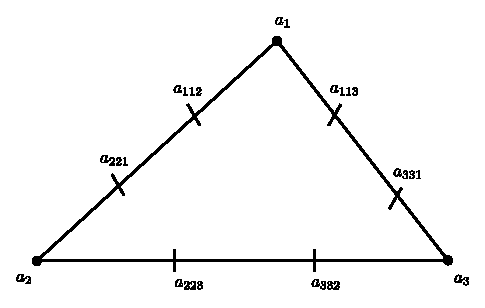
\includegraphics{figure/fig7.1.eps}
\caption{}\label{fig7.1}
\end{figure}

 In\pageoriginale fact, $\pi_h'$ is defined by 
$$
\int\limits_\gamma p(\pi_h'v).n\,ds=\int\limits_\gamma p(v.n)\,ds
\; \;\forall \;p\;\varepsilon\;\mathbb{P}_1(\gamma)
$$
However, the error estimates now become 
\begin{align*}
\parallel u-u_h\parallel_0 &\leq \ch^2\\
\parallel\lambda-\lambda_h\parallel_0 &\leq \ch
\end{align*}
\end{REM}

\begin{REM}\label{chap7:rem9}
The present finite element method can be extended to the elasticity
equation where $v$ represents the stress tensor $\sigma_{ij}$. The
difficulty lies in the required symmetry of $\sigma_{ij}$ but can be
surmounted. See C. JOHNSON-B. MERCIER \cite{key25} and
AMARA-THOMAS\cite{key2}. 
\end{REM}

\begin{REM}\label{chap7:rem10}
{\bf Aposteriori Error Estimate.} Let us consider the following
optimization problem:
\begin{align*}
&\Inf \;J(v,\mu)\\
&v\;\varepsilon \;Z(\phi)\\
&\mu\;\varepsilon \;M
\end{align*}
where $J(v,\mu)=1/2\parallel v-\nabla\mu\parallel^2$. Clearly the
optimal value is zero and corresponds to $v=u$ and $\mu=\lambda$
solution of \eqref{chap7:eq7.54}. Since $v\varepsilon Z(\phi)$, we
also have 
$$
J(v,\mu)=1/2\parallel\nabla\mu\parallel^2+(\phi,\mu)+1/2\parallel
v\parallel^2.
$$

Since $J(u,\lambda)\leq J(v_h,\lambda)\;\forall \;v_h\;\varepsilon
\;Z(\phi)$, we obtain
$$
1/2\parallel u\parallel^2\leq 1/2\parallel v_h\parallel^2.
$$\pageoriginale
Adding
$$
1/2\parallel\nabla\mu_h\parallel^2+(\phi,\mu_h)
$$
to both sides, where $\mu_h\varepsilon M$, we get 
$$
J(u,\mu_h)\leq J(v_h,\mu_h)\; \; \forall \;\mu_h\;\varepsilon \;M, \;v_h
\;\varepsilon \;Z(\phi).
$$
That is,
$$
\parallel\nabla(\lambda-\mu_h)\parallel_0\leq\parallel v_h-\nabla\mu_h
\parallel_0 \; \; \forall \;v_h\;\varepsilon \;Z(\phi).
$$

Suppose that $\mu_h$ is a solution of Dirichlet problem with a
conforming finite element method, then an upper bound for the error in
the energy norm is given by 
$$
\parallel v_h-\nabla\mu_h\parallel_0
$$
where
$$
v_h\;\varepsilon \;Z_h(\phi)
$$
is arbitrary. One can choose $v_h=u_h$, a solution of the present
equilibrium finite element approximation to Dirichlet problem.
\end{REM}

\section{Equilibrium Elements for the Plate
Problem} \label{chap7:ssec7.11}
 We recall that the equations of the
plate problem are:

Find $\sigma_{ij},w$ such that
\begin{align*}
\sigma_{ij}&=\lambda\Delta w\delta_{ij}+2\mu\frac{\partial^2w}
{\partial x_i\;\partial x_j}\;\text{in}\;\Omega\subset\mathbb{R}^2
\tag{7.57} \label{chap7:eq7.57}\\
\frac{\partial^2\sigma_{ij}}{\partial x_i\;\partial x_j} &=
f\;\text{in}\;\Omega \tag{7.57b} \label{chap7:eq7.57b}\\
w&= 0\;\text{on}\;\partial\Omega\tag{7.57c} \label{chap7:eq7.57c} 
\end{align*}\pageoriginale 
and 
\begin{equation*}
\begin{cases}
\frac{\partial w}{\partial n}=0\quad\text{on}\quad\partial\Omega
\quad\text{clamped case}\\
\sigma_{ij}\;n_i\;n_j=0\quad\text{on}\quad\partial\Omega\quad
\text{simply supported plate problem}\tag{7.57d}\label{chap7:eq7.57d}
\end{cases}
\end{equation*}
The summation convention is used in the above equations.

\begin{exercise}\label{chap7:exr6}
Show that \eqref{chap7:eq7.57} is equivalent to a biharmonic problem
for $w$ alone, and write the variational formulation of that
biharmonic problem. Notice that in the clamped case several bilinear
forms may be chosen unlike in the simply supported case.
\end{exercise}

It is easy to check that \eqref{chap7:eq7.57} is equivalent to 

\setcounter{equation}{57}
\begin{equation}\label{chap7:eq7.58}
\alpha\sigma_{ij}+\beta(\sigma_{kk})\;\delta_{ij}= \frac{\partial^2w}
{\partial x_i\;\partial x_j},
\end{equation}
where
$$
\alpha=1/2\mu\quad\text{and}\quad\beta=\frac{-\lambda}
{2\mu(2\lambda+2\mu)}.
$$

Let 
$$
a(\sigma,\tau)=\int\limits_\Omega(\alpha\sigma_{ij}\tau_{ij}+
\beta(\sigma_{kk})(\tau_{\ell\ell}))\,dx
$$
and 
$$
Dw=\left(\frac{\partial^2w}{\partial x_i\;\partial x_j}\right).
$$
Then\pageoriginale problem \eqref{chap7:eq7.57} is equivalent to:
\begin{align*}
&\text{Find}\quad\sigma\varepsilon \;(L^2(\Omega))_s^4,\;w\;\varepsilon
\;H_\circ^2(\Omega)\quad\text{such that}\\
&a(\sigma,\tau)-\int\limits_\Omega\tau \;Dw\,dx=0\; \; \forall
\;\tau\varepsilon \;(L^2(\Omega))_s^4,\\
&\int\limits_\Omega\sigma \;Dv=\int\limits_\Omega fv\,dx. \;\forall 
\begin{cases}
v\;\varepsilon \;H_\circ^2(\Omega).\\
v\;\varepsilon \;H^2(\Omega)\cap \;H_\circ^1(\Omega).
\end{cases}
\end{align*}
$(L^2(\Omega))_s^4$ denotes the set of symmetric $2\times 2$ tensors
which are in $L^2(\Omega)$.

However, as noticed in Section \ref{chap7:ssec7.10}, to approximate this problem 
in the usual way does not represent any progress on the usual conforming
approximations since one has to approximate $H_\circ^2(\Omega)$. 

We have, by Green's formula,
\begin{align*}
\int\limits_K\tau \;Dv &= \int\limits_K\tau_{ij} \frac{\partial^2v}
{\partial x_i\partial x_j}\,dx\\
&= \int\limits_{\partial K}\tau_{ij}\;n_j\frac{\partial v}{\partial
x_i}-\int\limits_K \frac{\partial\tau_{ij}}{\partial x_j}
\frac{\partial v}{\partial x_i}\,dx
\end{align*}
Since
$$
\frac{\partial v}{\partial x_i}=\frac{\partial v}{\partial n}n_i+
\frac{\partial v}{\partial s}s_i
$$
where $(s_i)$ are the components of the unit tangent vector, we obtain
$$
\int\limits_\Omega\tau \;Dv=\sum\limits_K\int\limits_{\partial K}M_n
(\tau)\frac{\partial v}{\partial n}+\sum\limits_K\left(
\int\limits_{\partial K}M_{ns}(\tau)\frac{\partial v} {\partial s}-
\int\limits_K\frac{\partial\tau_{ij}}{\partial x_j} \frac{\partial v}
{\partial x_i}\,dx\right)
$$
Here 
$$
M_n(\tau)=\tau_{ij}\;n_i\;n_j,\;M_{ns}(\tau)=\tau_{ij}\;n_j\;s_i.
$$\pageoriginale
We define
\begin{align*}
&b(\tau,v)=\sum\limits_K\left(\int\limits_K\frac{\partial\tau_{ij}}
{\partial x_j}\;\frac{\partial v}{\partial x_i}\,dx-
\int\limits_{\partial K}M_{ns}(\tau)\frac{\partial v} {\partial s}
\,ds\right), \\
&V=\{\tau:\tau|_K\;\varepsilon \;(H^1(K))_s^4,\;K\;\varepsilon \;T_h,
M_n(\tau) 
\end{align*}
is continuous across inter element boundaries\}.

Then 
$$
\int\limits_\Omega\tau \;Dv=b(v,\tau)\; \; \forall \;v\;\varepsilon
\;H_\circ^2(\Omega), \;\tau \;\varepsilon \;V.
$$

In fact, $b(\cdotp,\cdotp)$ is continuous over $V\times M$ where
$M=W_\circ^{1,p}(\Omega)(p>2)$ so that \eqref{chap7:eq7.57} (clamped
case) is equivalent to:

Find $\{\sigma,w\}\;\varepsilon \;V\times M$ such that 
\begin{equation}\label{chap7:eq7.59}
\begin{aligned}
&a(\sigma,\tau)+b(\tau,w)=0\; \; \forall \;\tau \;\varepsilon \;V,\\
&b(\sigma,v)=-(f,v)\; \; \forall \;v\;\varepsilon \;M.
\end{aligned}
\end{equation}
We take 
$$
H=(L^2(\Omega))_s^4.
$$

The Brezzi condition holds only on $H_\circ^1(\Omega)$, since if $v$
is smooth and $\tau_{ij}=v\delta_{ij}$, then 
\begin{align*}
M_{ns}(\tau) &= v\;(\delta_{ij}\;n_j\;s_i)=0,\\
M_n(\tau) &= v,
\end{align*}
and\pageoriginale
$$
b(v,\tau)=\int\limits_\Omega|\nabla v|^2\,dx\geq\alpha\parallel
v\parallel_1^2\geq c\parallel v\parallel_1\parallel\tau\parallel.
$$

For the proof of existence of solutions of \eqref{chap7:eq7.59} and
modified error estimates see BREZZI-RAVIART \cite{key7}.

We choose 
$$
V_h=\{\tau:\tau\;\varepsilon \;(\mathbb{P}_\circ(K))_s^4,\;K\;
\varepsilon \;T_h,\;M_n(\tau)\quad\text{is continuous}\}.
$$

Since
$$
v\;\varepsilon \;W_\circ^{1,p}(\Omega)\subset
\;C^\circ(\overline{\Omega})
$$
we find that after integration by parts on each of $\partial
K,\;b(\tau,v)$ involves only the values of $v$ at the vertices of
$T_h$:
\begin{equation*}\label{chap7:eq7.59b}
b(\tau,v)=\sum\limits_K\int\limits_{\partial K}M_{ns}(\tau)
\frac{\partial v}{\partial s}=\sum\limits_NR(\tau,N)\;v(N)\; \; \forall
\;\tau \;\varepsilon \;V_h.\tag{7.59b}
\end{equation*}

Notice that only the value of $v$ at the vertices has to be taken;
therefore, we choose
$$
M_h=\left\{v_h\;\varepsilon \;C^\circ(\overline{\Omega}):\;v_h|_K\;
\varepsilon \;\mathbb{P}_1(K),K\;\varepsilon \;T_h,\;v_h=0\quad
\text{on}\quad\partial\Omega\right\}
$$
so that, if $\tau \varepsilon V_h$, then 
$$
b(\tau,v_h)=0 \; \;\forall \;v_h\;\varepsilon \;M_h\Rightarrow b(\tau,v)=0
\; \;\forall \;v\;\varepsilon \;M.
$$
Therefore, $Z_h(0)\subset Z(0)$. Hence 
$$
\parallel\sigma -\sigma_h\parallel_0\leq \underset{\tau_h\varepsilon
Z_h(-f)}{\Inf}\parallel\sigma -\tau_h\parallel.
$$
Here $\{\sigma_h,w_h\}\varepsilon V_h\times M_h$ is the solution of
the approximate problem. 
\begin{equation}\label{chap7:eq7.60}
\begin{cases}
a(\sigma_h,\tau_h)+\Sigma \;R(\tau_h,N)\;w_h(N)=0\; \; \forall \;\tau_h
\;\varepsilon \;V_h,\\
\Sigma \;R(\sigma_h,N)\;v_h(N)=-(f,v_h)\; \; \forall \;v_h\;\varepsilon \;M_h
\end{cases}
\end{equation}\pageoriginale 

\subsubsection{\bf Interpolation Operator.} The interpolation operator 
$$
\pi_h:\;(H^1(\Omega))^4\to V_h
$$
is defined by
$$
\int\limits_\gamma M_n(\pi_h,\sigma)\,ds=\int\limits_\gamma
M_n(\sigma)\,ds,
$$
for each edge $\gamma$ of the triangulation. 

We have the estimate

\begin{THM}\label{chap7:THM12}
There exists a constant $c$ independent of $h$ such that 
\begin{equation}\label{chap7:eq7.61}
\parallel\pi_hv\parallel_V\leq c\parallel v\parallel_V
\end{equation}
and 
\begin{equation}\label{chap7:eq7.62}
\parallel\pi_hv-v\parallel_{0,\Omega}\leq\ch\parallel v
\parallel_{1.\Omega}\; \; \forall \;v\;\varepsilon \;(H^1(\Omega))^4.
\end{equation}

The proof of this is found in C.JOHNSON \cite{key24}.
\end{THM}

\subsubsection{\bf Properties of $T_h$.} We have 
\begin{align*}
b(\pi_h\sigma,v_h) &= \sum\limits_K\int\limits_{\partial K}M_n
(\pi_h\sigma)\frac{\partial v_h}{\partial n}- \int\limits_K
(\pi_h\sigma)\;D\;v_h\\
&= \sum\limits_K\int\limits_{\partial K}M_n(\sigma) \frac{\partial
v_h}{\partial n},\;\forall \;v_h \;\varepsilon \;M_h\\
&= b(\sigma, v_h).
\end{align*}
Hence\pageoriginale
\begin{equation}\label{chap7:eq7.63}
b(\pi_h\sigma -\sigma,v_h)=0\; \;\forall \;v_h\;\varepsilon \;M_h 
\end{equation}
Therefore $\pi_h$ maps $Z(\phi)$ into $Z_h(\phi)$.

Equations \eqref{chap7:eq7.61} and \eqref{chap7:eq7.63} imply that the
discrete Brezzi condition is satisfied.

We have the error estimate
$$
\parallel w-w_h\parallel_1\leq c\left(\parallel\sigma-
\sigma_h\parallel_0+\underset{v_h\varepsilon M_h}{\Inf}\parallel
w-v_h\parallel_{1,p}\right) 
$$
(See BREZZI-RAVIART \cite{key7}).

The above method is called Hermann-Johnson method.

\subsubsection{\bf Morley Nonconforming Method.} Let 

$W_h=\{v_h:v_h|_K\;\varepsilon \;\mathbb{P}_2(K),\;K\;\varepsilon
\;T_h$,
\begin{align*}
&v_h\quad\text{continuous at the vertices},\\
&\frac{\partial v_h}{\partial n}\quad\text{continuous at the mid side
point},\\
&v_h=0\quad\text{at the boundary vertices},\\
&\frac{\partial v_h}{\partial n}=0\quad\text{at the mid point of
boundary edges}\}
\end{align*}

The space $W_h$ makes use of the Morley finite element which has 6
degrees of freedom, namely, values at the three vertices and the
values of the normal derivatives at the three mid side points.
\begin{figure}[H]
\centering
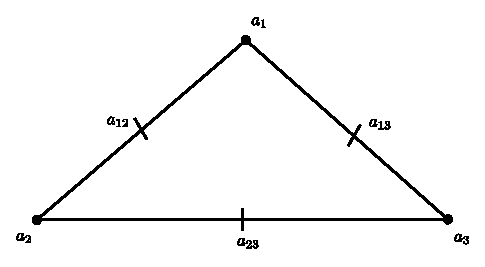
\includegraphics{figure/fig7.2.eps}
\caption{}\label{fig7.2}
\end{figure}\pageoriginale

We consider, for simplicity, the case $\lambda=0$ and $\mu=1/2$ so
that
$$
a(\sigma,\tau)=\int\limits_\Omega \tau_{ij}\;\sigma_{ij}\,dx.
$$
Let
$$
L(v)=\sum\limits_N f_N\;v(N);
$$
that is $L$ is a linear combination of Dirac masses (concentrated
loads). Then 

\begin{THM}\label{chap7:THM13}
The problem:

Find $u_h\varepsilon W_h$ such that 
\begin{equation}\label{chap7:eq7.64}
\sum\limits_K\int\limits_K D\;u_h \;D\;v_h\,dx=L(v_h)\;\; \forall \;v_h
\;\varepsilon \;W_h,
\end{equation}
is equivalent to \eqref{chap7:eq7.60} when 
$$
(f,v)=\sum\limits_N f_N\;v(N)
$$
in the sense that 
$$
u_h(N)=W_h(N)\quad\text{at the vertices}\quad N,
$$
and 
$$
\sigma_h|_K=Du_h|_K,\;K\;\varepsilon \;T_h.
$$
\end{THM}
\begin{proof}
Let\pageoriginale $u_h$ be a solution of \eqref{chap7:eq7.64}.

Define
$$
\sigma_h^*|_K=Du_h|_K\quad\text{and}\quad w_h^*\varepsilon M_h\quad
\text{by}\quad w_h^*(N)=u_h(N).
$$
We will show that $\{\sigma_h^*(N),w_h^*\}$ is the solution of
\eqref{chap7:eq7.60}. Since $u_h$ is a solution \eqref{chap7:eq7.64},
we have 
\begin{equation}\label{chap7:eq7.65}
\sum\limits_K\int\limits_K\sigma_h^*\;Dv_h\,dx=L(v_h)\; \; \forall \;v_h\;
\varepsilon \;W_h
\end{equation}
Using Green's formula, we obtain 
\begin{equation}\label{chap7:eq7.66}
\sum\limits_K\left(\int\limits_{\partial K}\;M_n(\sigma_h^*)
\frac{\partial v_h}{\partial n}+\int\limits_{\partial K}M_{ns}
(\sigma_h^*)\frac{\partial v_h}{\partial s}\right)=L(v_h)\; \; \forall
\;v_h \;\varepsilon \;W_h
\end{equation}

If $b_i$ is one mid side point, then substituting $v_h$ satisfying:
\begin{align*}
&v_h=0\quad\text{at the vertices}\\
&\frac{\partial v_h}{\partial n}=
\begin{cases}
1\quad\text{at}\quad b_i\\
0\quad\text{at the other nodes}\quad b_j,\;j\neq i
\end{cases}
\end{align*}
in the above equation we obtain that $M_n(\sigma_h^*)$ is continuous
at $b_i$ (by using \ref{chap7:eq7.59b}). This proves that
$\underset{h}{*}\varepsilon V_h$.

Since $\sigma_h^* \varepsilon V_h$, equation \eqref{chap7:eq7.66}
gives 
$$
\sum\limits_K\int\limits_{\partial K}\;M_{ns}(\sigma_h^*)
\frac{\partial v_h}{\partial s}=\sum\limits_Nf_Nv_h(N)\; \; \forall \;v_h
\;\varepsilon \;W_h
$$
But 
$$
\sum\limits_K\int\limits_KM_{ns}(\sigma_h^*)\frac{\partial v_h}
{\partial s}=-\sum\limits_NR(\sigma_h^*,\;N)\;v_h(N).
$$
Hence\pageoriginale
\begin{equation}\label{chap7:eq7.67}
\sum\limits_KR(\sigma_h^*,N)\;v_h(N)=-\sum\limits_Nf_N\;v_h(N)\; \; \forall
\;v_h \;\varepsilon \;W_h.
\end{equation}
Let $v_h\varepsilon M_h$. Consider $\tilde{v}_h\varepsilon V_h$
defined by 
$$
\tilde{v}_h(N)=v_h(N),\frac{\partial}{\partial n}\;\tilde{v}_h
(b_i)=0.
$$
Then \eqref{chap7:eq7.67} gives
$$
\sum\limits_KR(\sigma_h^*,N)\;\tilde{v}_h(N)=-\sum\limits_Nf_N
\;\tilde{v}_h(N) 
$$
Therefore 
$$
\sum\limits_NR(\sigma_h^*,N)\;v_h(N)=-\sum\limits_Nf_N\;v_h(N)\; \; \forall
\;v_h \;\varepsilon \;M_h.
$$
This is nothing but the second equation in \eqref{chap7:eq7.60} with
$\sigma_h$ replaced by $\sigma_h^*$. Now
\begin{align*}
a(\sigma_h^*,\tau) &= \sum\limits_K\int\limits_K\;(\sigma_h^*)_{ij}\;
\tau_{ij}\\ 
&= \sum\limits_K\int\limits_K\frac{\partial^2u_h}{\partial x_i\;
\partial x_j}\;\tau_{ij}\\
&= \sum\limits_K\int\limits_KM_n(\tau)\frac{\partial u_h}{\partial n}
+\int\limits_KM_{ns}(\tau)\frac{\partial u_h}{\partial s} \; \; \forall
\;\tau \;\varepsilon \;V_h
\end{align*}
by Green's formula.

The first term in the right side is zero since $u_h\varepsilon W_h$
and $\tau\varepsilon V_h$. The second term equals
$-\sum\limits_NR(\tau,N)u_h(N)$. Hence we obtain 
$$
a(\sigma_h^*,\tau)+\sum\limits_NR(\tau,N)\;w_h^*(N)=0\; \; \forall \;\tau
\;\varepsilon \;V_h,
$$
since $u_h(N)=w_h^*(N)$. 

Thus\pageoriginale $\{\sigma_h^*,w_h^*\}$ is a solution of
\eqref{chap7:eq7.60}. By uniqueness we have $\sigma_h=\sigma_h^*$ and
$w_h^*=w_h$. 

Thus we have proved that \eqref{chap7:eq7.64} $\Rightarrow$
\eqref{chap7:eq7.60}. Let $\{\sigma_h,w_h\}$ be the solution of
\eqref{chap7:eq7.60}. We will show that $u_h$ defined by 
\begin{align}
u_h(N) &= w_h(N)\quad\text{for each vertex}\quad
N \label{chap7:eq7.68}\\
Du_h|_K &= \sigma_h|_K\quad\text{for each}\quad K\;\varepsilon
\;T_h \label{chap7:eq7.69} 
\end{align}
is the solution of \eqref{chap7:eq7.64}.

It is easy to see that \eqref{chap7:eq7.68} and \eqref{chap7:eq7.69}
define a unique $u_h$ such that $u_h|_K\;\varepsilon\;\mathbb{P}_2(K)$
for each $K\varepsilon T_h$. We will prove that this $u_h\varepsilon
W_h$. 

From the first equation in \eqref{chap7:eq7.60}, we obtain
$$
\sum\limits_K\int\limits_{\partial K}M_n(\tau)\frac{\partial u_h}
{\partial n}=0\; \; 
\forall \;\tau \;\varepsilon \;V_h.
$$

This implies $\partial u_h/\partial n$ is continuous at mid side
points and $\partial u_h/\partial n=0$ at the boundary mid side
points. Hence $u_h\varepsilon W_h$.

Let $v_h\varepsilon W_h$. Then there exists $v_h\varepsilon M_h$ such
that $\tilde{v}_h(N)=v_h(N)$. Hence the second equation in
\eqref{chap7:eq7.60} gives
$$
\sum R(\sigma_h,\;N)\;v_h(N)=-\sum f_N\;v_h(N).
$$
This shows
$$
\sum\limits_K\int\limits_K Du_h\;Dv_h=\sum\limits_N f_N\;v_h.
$$
This proves \eqref{chap7:eq7.60} $\Rightarrow$ \eqref{chap7:eq7.64}.

Thus\pageoriginale the Hermann-Johnson method and the Morley
nonconforming method are equivalent, in this particular case where the
load is a sum of concentrated loads. 
\end{proof}

\begin{exercise}\label{chap7:exr7}
Let $K$ be a triangle. Let $\mathbb{P}_K=\mathbb{P}_2(K)$ and 
$$
\sum_K=\left\{\delta_{a_i},\frac{\partial}{\partial n}\delta_{a_{ij}},1\leq
i< j\leq 3\right\},
$$
where $a_i$'s denote the vertices of $K$ and $a_{ij}$'s denote the mid
points of the sides of $K$. Show that $\sum_K$ is
$\mathbb{P}_K$-unisolvent. The above finite element is called the
Morley finite element.
\begin{figure}[H]
\centering
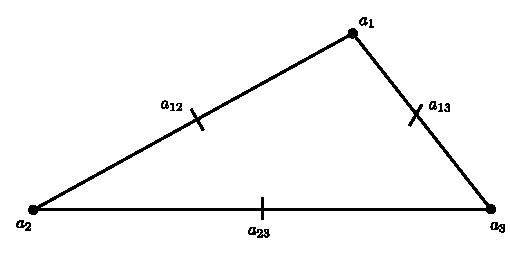
\includegraphics{figure/fig7.3.eps}
\caption{}\label{fig7.3}
\end{figure}
\end{exercise}

\begin{REM}\label{chap7:rem11}
We note that the Morley element has advantage over Herrmann-Johnson
method, since in Morley's method we get a positive definite matrix and
we have no constraints. 
\end{REM}






